% ============================================================================
%  CV Assignment 1 — Panorama Stitching Report
%  IEEE Conference Template
% ============================================================================
\documentclass[conference]{IEEEtran}

% ── Packages ───────────────────────────────────────────────────────────────
\usepackage[utf8]{inputenc}
\usepackage[T1]{fontenc}
\usepackage{amsmath,amssymb,amsfonts}
\usepackage{graphicx}
\usepackage[caption=false,font=footnotesize]{subfig}

% Keep subfloats self-contained so captions don't leak/float weirdly.
\captionsetup[subfloat]{farskip=0pt,captopadj=0pt}
\usepackage{booktabs}
\usepackage{hyperref}
\usepackage{algorithm}
\usepackage{algpseudocode}
\usepackage{xcolor}
\usepackage{listings}
\usepackage{float} % avoid using [H] for IEEE (use [!t]/[!b] instead)
\usepackage{url}
\usepackage{microtype}
\usepackage{bookmark}
\usepackage[section]{placeins}

% (Use subfig's \subfloat{...}; do not use the subfigure environment.)

% ── Listing style ──────────────────────────────────────────────────────────
\lstset{
  language=Python,
  basicstyle=\ttfamily\footnotesize,
  keywordstyle=\color{blue}\bfseries,
  commentstyle=\color{green!60!black},
  stringstyle=\color{red!70!black},
  breaklines=true,
  frame=single,
  captionpos=b,
}

% ── Graphics path ──────────────────────────────────────────────────────────
% Images live in this project under Assignment - 1/output/
\graphicspath{{output/}}

% ── Title ──────────────────────────────────────────────────────────────────
\title{Assignment - 1}

\author{
  \IEEEauthorblockN{Madhav Kataria}
  \IEEEauthorblockA{
    Roll No: B23CH1025 \\
    Email: b23ch1025@iitj.ac.in
  }
}

\begin{document}

\maketitle

% ═══════════════════════════════════════════════════════════════════════════
%   ABSTRACT
% ═══════════════════════════════════════════════════════════════════════════
\begin{abstract}
This report presents an image stitching pipeline that constructs panoramic
images from multiple overlapping photographs. The system uses Scale-Invariant
Feature Transform (SIFT) for keypoint detection and descriptors, FLANN-based
matching with Lowe's ratio test for correspondences, and robust homography
estimation for global alignment. To address strong ghosting in challenging
parallax scenes, we add two practical refinements: (1) post-warp
ECC-based local alignment to the centre image, and (2) adaptive deghost
blending based on seam ownership (label assignment) with narrow feathering.
We also include cylindrical warping to reduce wide-angle edge distortion.
Experiments show that the proposed refinements significantly reduce double
edges and seam visibility on difficult real-world captures while preserving
quality on easy scenes.
\end{abstract}

\begin{IEEEkeywords}
Panorama stitching, SIFT, homography, RANSAC, multi-band blending,
Laplacian pyramid, cylindrical warping, ECC alignment, deghosting
\end{IEEEkeywords}


% ═══════════════════════════════════════════════════════════════════════════
%   1. INTRODUCTION
% ═══════════════════════════════════════════════════════════════════════════
\section{Introduction}

Image mosaicking, or panorama stitching, is a fundamental problem in computer
vision that involves combining multiple images with overlapping fields of view
into a single, wide-angle composite image. Applications range from consumer
photography (e.g., smartphone panorama modes) to medical imaging, satellite
imagery, and virtual reality environment capture.

The general pipeline for panorama construction consists of four stages:
\begin{enumerate}
  \item \textbf{Feature Detection and Description:} Identifying salient
        interest points in each image and computing local descriptors that are
        invariant to scale, rotation, and (partially) illumination changes.
  \item \textbf{Feature Matching:} Establishing correspondences between
        features in overlapping image pairs.
  \item \textbf{Geometric Estimation:} Computing the projective transformation
        (homography) that maps one image into the coordinate frame of another.
  \item \textbf{Warping and Blending:} Transforming all images onto a common
        canvas and merging them seamlessly.
\end{enumerate}

In this work, we implement the full pipeline using well-established
algorithms—SIFT~\cite{lowe2004}, FLANN~\cite{muja2009},
RANSAC~\cite{fischler1981}—and investigate three advanced techniques to
improve the output quality:
\begin{itemize}
  \item \textbf{Multi-band blending} via Laplacian pyramids~\cite{burt1983},
        which blends different frequency components at different spatial scales.
  \item \textbf{Cylindrical warping}~\cite{szeliski2006}, which projects
        images onto a cylindrical surface to reduce edge distortion.
  \item \textbf{ECC refinement + adaptive deghost blending}, which performs
        local post-warp registration and overlap-aware seam ownership to
        suppress visible double edges in parallax-heavy scenes.
\end{itemize}

Our work follows the automatic panorama framework of Brown and
Lowe~\cite{brown2007} and the projective geometry foundations in Hartley and
Zisserman~\cite{hartley2003}.

The remainder of this report is organised as follows: Section~\ref{sec:method}
describes each component of the pipeline in detail; Section~\ref{sec:novel}
presents the novel techniques; Section~\ref{sec:results} shows experimental
results with qualitative and quantitative comparisons; Section~\ref{sec:code}
discusses the software architecture; and Section~\ref{sec:conclusion}
concludes this report.

\subsection*{Pipeline Overview}

Figure~\ref{fig:pipeline} illustrates the overall panorama stitching workflow.
The standard SIFT path and cylindrical path share a common warping and
blending backend. In the updated pipeline, warped images are locally refined
with ECC before blending, and overlap disagreement triggers stronger deghost
seam assignment.

\begin{figure}[!htbp]
  \centering
  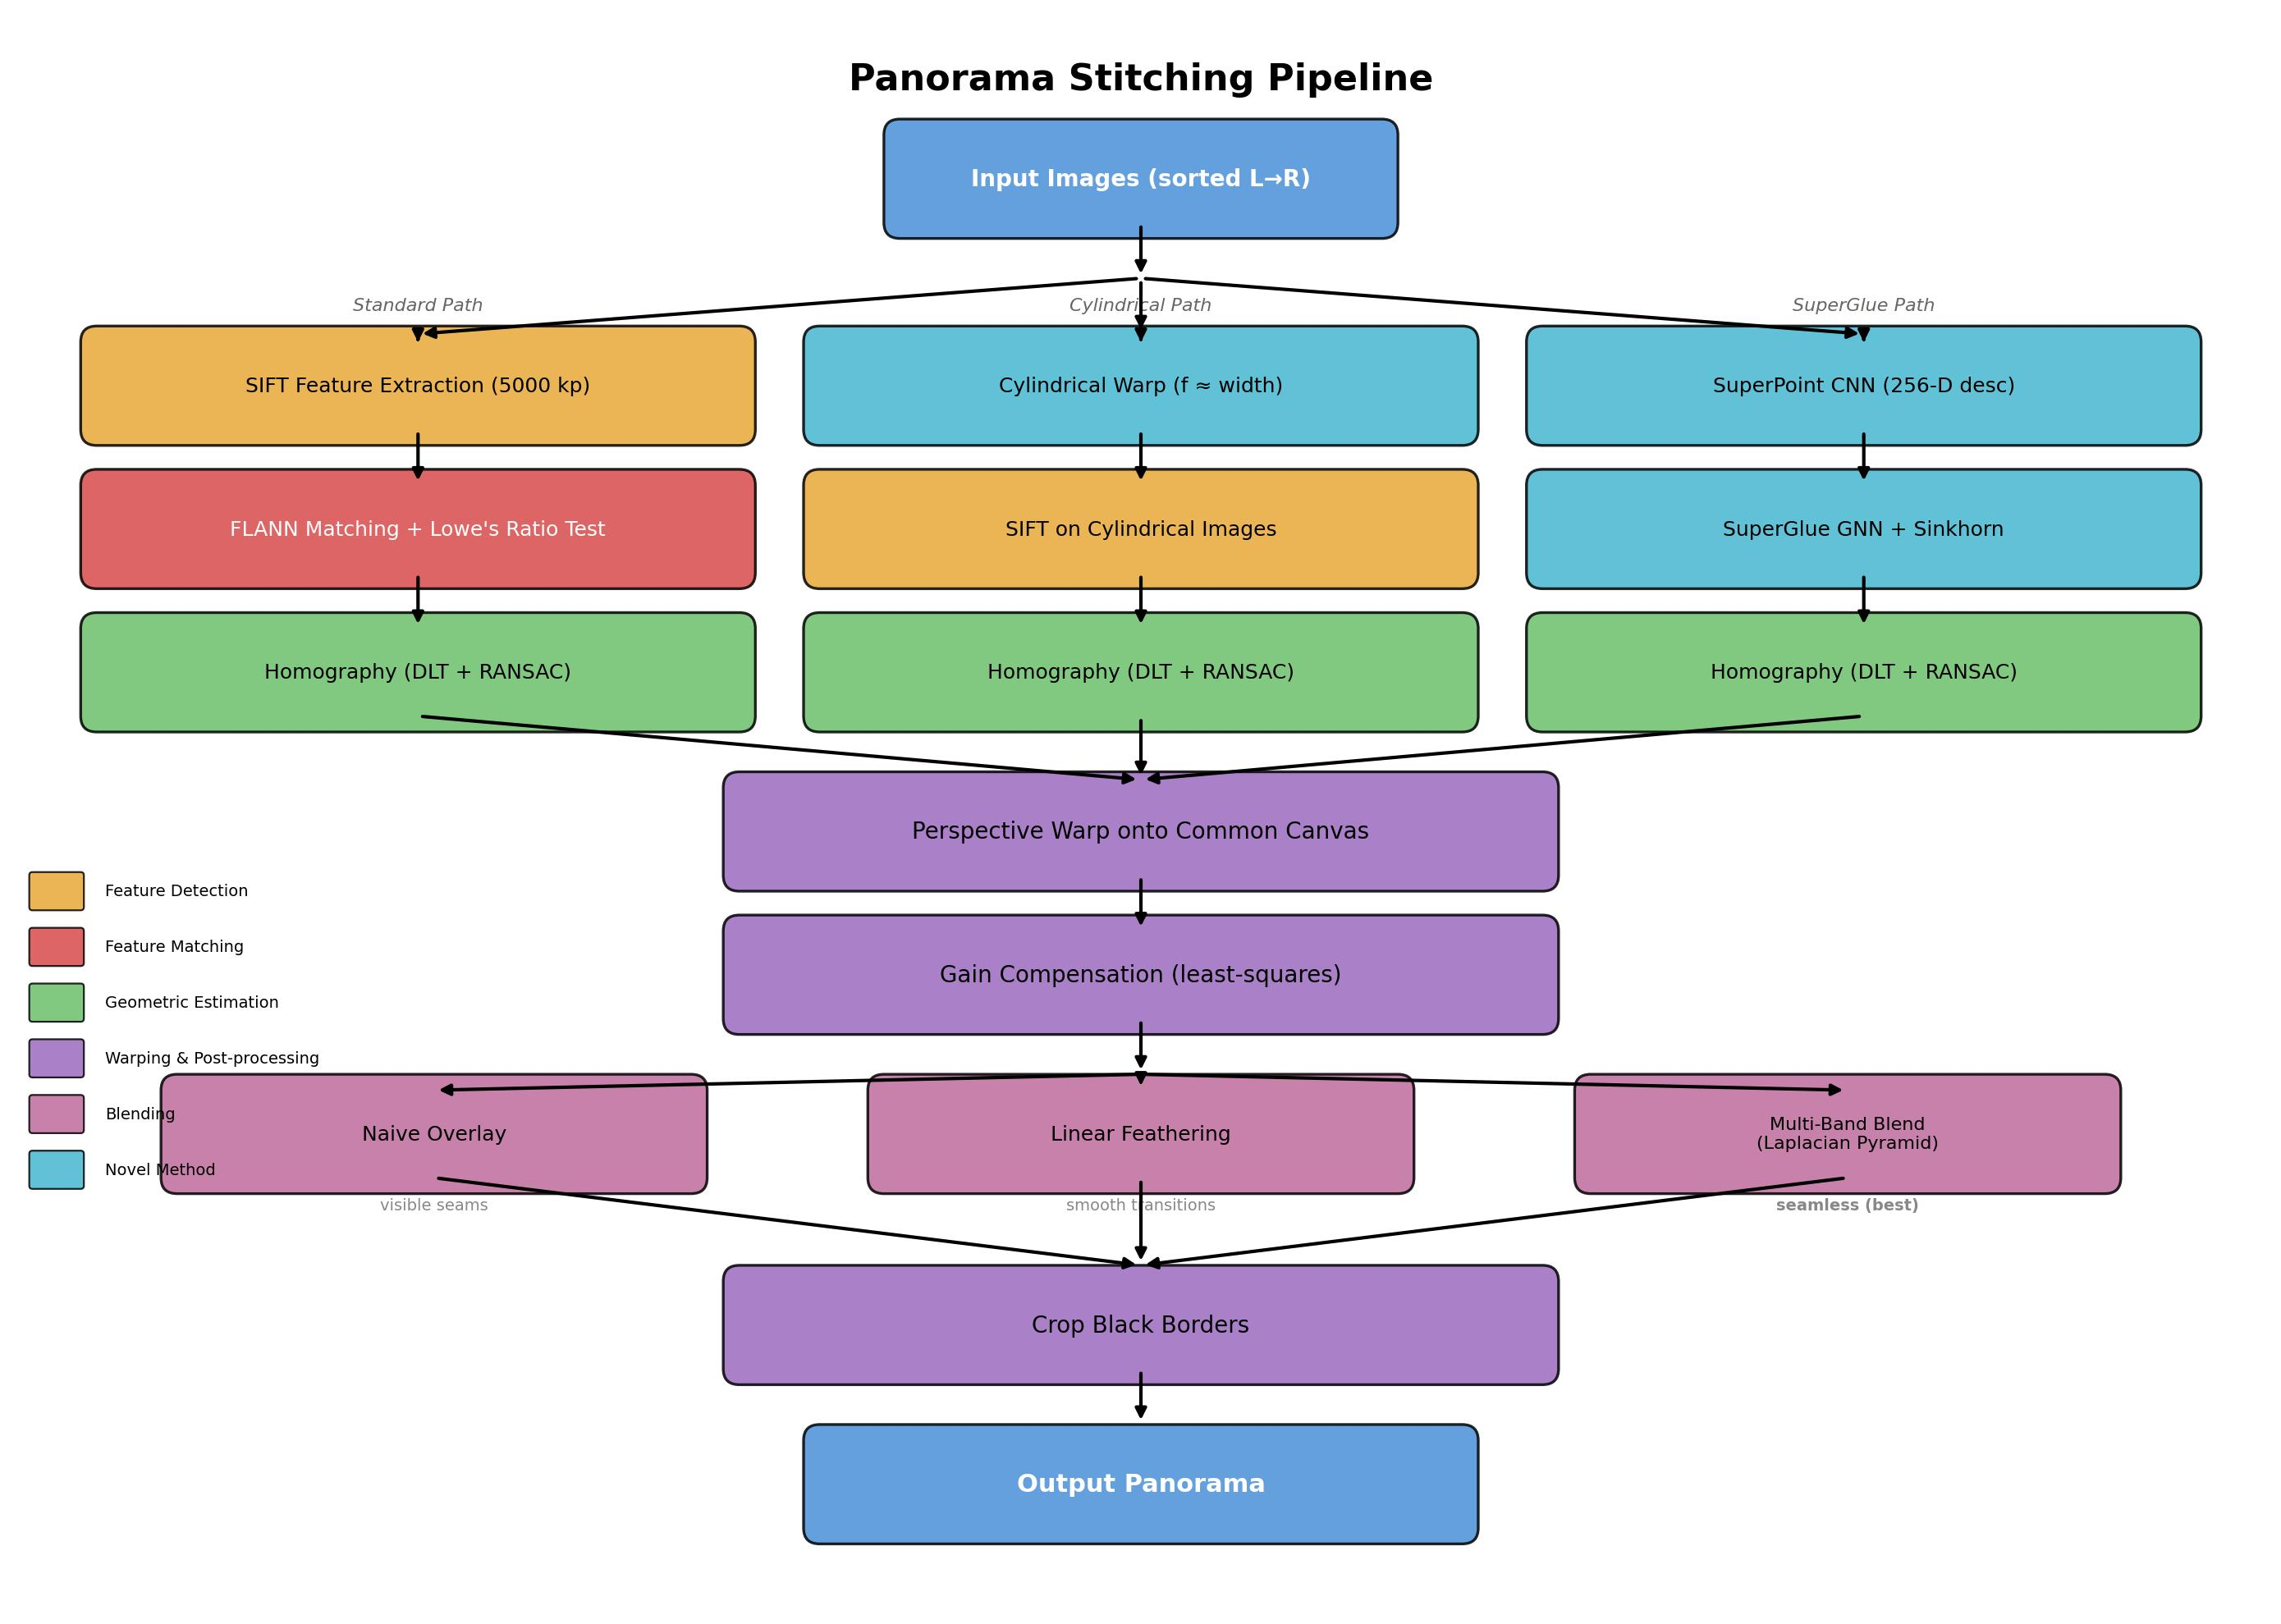
\includegraphics[width=\linewidth]{pipeline_diagram.jpg}
  \caption{Full panorama stitching pipeline. Standard and cylindrical branches
           feed a common warping, ECC refinement, gain compensation, and
           adaptive blending stage.}
  \label{fig:pipeline}
\end{figure}


% ═══════════════════════════════════════════════════════════════════════════
%   2. METHODOLOGY
% ═══════════════════════════════════════════════════════════════════════════
\section{Methodology}
\label{sec:method}

% ── 2.1 SIFT ──────────────────────────────────────────────────────────────
\subsection{SIFT Feature Extraction}

The Scale-Invariant Feature Transform (SIFT), proposed by Lowe~\cite{lowe2004},
detects keypoints that are invariant to scaling, rotation, and partially
invariant to affine transformations and illumination changes. The algorithm
proceeds in four stages:

\subsubsection{Scale-Space Extrema Detection}
A Gaussian scale-space is constructed by convolving the input image $I(x,y)$
with Gaussian kernels of increasing standard deviation $\sigma$:
\begin{equation}
  L(x, y, \sigma) = G(x, y, \sigma) * I(x, y)
\end{equation}
where $G(x, y, \sigma) = \frac{1}{2\pi\sigma^2}
\exp\!\left(-\frac{x^2 + y^2}{2\sigma^2}\right)$.

Difference-of-Gaussian (DoG) images approximate the scale-normalised
Laplacian $\sigma^2 \nabla^2 G$:
\begin{equation}
  D(x, y, \sigma) = L(x, y, k\sigma) - L(x, y, \sigma)
\end{equation}
Keypoint candidates are located at local extrema of $D$ across both spatial
coordinates and scale.

\subsubsection{Keypoint Localisation}
Sub-pixel and sub-scale accuracy is achieved by fitting a 3D quadratic to the
DoG values around each candidate:
\begin{equation}
  D(\mathbf{x}) \approx D + \frac{\partial D^T}{\partial \mathbf{x}} \mathbf{x}
  + \frac{1}{2} \mathbf{x}^T \frac{\partial^2 D}{\partial \mathbf{x}^2} \mathbf{x}
\end{equation}
Candidates with low contrast ($|D(\hat{\mathbf{x}})| < 0.03$) or strong edge
response (ratio of principal curvatures $> 10$) are discarded.

\subsubsection{Orientation Assignment}
For each surviving keypoint, a histogram of gradient orientations in a
neighbourhood weighted by $\sigma$ is computed. The dominant peak(s) determine
the keypoint orientation(s), making the descriptor rotation-invariant.

\subsubsection{Descriptor Computation}
A $16 \times 16$ patch around the keypoint (rotated to the dominant
orientation) is divided into a $4 \times 4$ grid of sub-regions. In each
sub-region, an 8-bin orientation histogram is computed, yielding a
$4 \times 4 \times 8 = 128$-dimensional descriptor vector, normalised to
unit length for illumination invariance.

In our implementation we use OpenCV's \texttt{cv2.SIFT\_create(nfeatures=10000)},
extracting up to 10,000 keypoints per image.

% ── 2.2 Matching ─────────────────────────────────────────────────────────
\subsection{Feature Matching}

Given descriptor sets $\{d_i^A\}$ and $\{d_j^B\}$ from two images, we seek
correspondences using approximate nearest-neighbour search.

\subsubsection{FLANN Matcher}
The Fast Library for Approximate Nearest Neighbours (FLANN)~\cite{muja2009}
constructs a KD-tree index over the descriptor space, enabling $k$-NN queries
in $O(D \log N)$ time rather than the brute-force $O(DN)$, where $D=128$ is
the descriptor dimensionality and $N$ is the number of features.

\subsubsection{Lowe's Ratio Test}
To reject ambiguous matches, we apply Lowe's ratio test~\cite{lowe2004}:
a match $(m, n)$ from a $k=2$ nearest-neighbour query is kept only if
\begin{equation}
  \frac{\|d_i^A - d_m^B\|}{\|d_i^A - d_n^B\|} < \tau
\end{equation}
where $\tau = 0.70$ is the ratio threshold. This eliminates features near
decision boundaries where multiple descriptors are similarly close.

% ── 2.3 Homography ───────────────────────────────────────────────────────
\subsection{Homography Estimation}

A homography $\mathbf{H} \in \mathbb{R}^{3 \times 3}$ is a projective
transformation between two planes. Given corresponding points
$\mathbf{p} = (x, y, 1)^T$ and $\mathbf{p}' = (x', y', 1)^T$:
\begin{equation}
  s \begin{pmatrix} x' \\ y' \\ 1 \end{pmatrix}
  = \begin{pmatrix} h_{11} & h_{12} & h_{13} \\
                     h_{21} & h_{22} & h_{23} \\
                     h_{31} & h_{32} & h_{33} \end{pmatrix}
    \begin{pmatrix} x \\ y \\ 1 \end{pmatrix}
  \label{eq:homography}
\end{equation}
where $s$ is an arbitrary scale factor. Normalising $h_{33} = 1$, $\mathbf{H}$
has 8 degrees of freedom. Each point correspondence provides 2 equations, so a
minimum of \textbf{4 non-collinear correspondences} are needed to determine
$\mathbf{H}$ via the Direct Linear Transform (DLT).

\subsubsection{DLT Algorithm}
Each correspondence $(x_i, y_i) \leftrightarrow (x_i', y_i')$ contributes two
rows to the system $\mathbf{A}\mathbf{h} = \mathbf{0}$:
\begin{equation}
  \begin{pmatrix}
    -x_i & -y_i & -1 & 0 & 0 & 0 & x_i'x_i & x_i'y_i & x_i' \\
    0 & 0 & 0 & -x_i & -y_i & -1 & y_i'x_i & y_i'y_i & y_i'
  \end{pmatrix}
\end{equation}
The solution $\mathbf{h}$ is the right singular vector of $\mathbf{A}$
corresponding to the smallest singular value (via SVD).

\subsubsection{RANSAC}
\label{sec:ransac}
Feature matches inevitably contain outliers. RANSAC (Random Sample Consensus)
~\cite{fischler1981} robustly estimates $\mathbf{H}$ by iteratively:
\begin{enumerate}
  \item Randomly sampling 4 correspondences.
  \item Computing $\mathbf{H}$ from these 4 points via DLT.
  \item For every other correspondence, computing the reprojection error
        $\epsilon_i = \|\mathbf{p}_i' - \mathbf{H}\mathbf{p}_i\|_2$. If
        $\epsilon_i < \tau_{\text{RANSAC}}$ (we use $\tau_{\text{RANSAC}} = 1.5$ px),
        the match is classified as an inlier.
  \item After $N$ iterations, refitting $\mathbf{H}$ using \emph{all} inliers
        from the best iteration.
\end{enumerate}

Practically, we use OpenCV's USAC\_MAGSAC estimator in a two-stage refinement:
an initial robust fit at 1.5 px, followed by re-estimation on inliers at a
tighter threshold. A final LMEDS polish is applied when sufficient inliers
remain.

The number of iterations is determined by:
\begin{equation}
  N = \frac{\log(1 - p)}{\log(1 - w^n)}
\end{equation}
where $p = 0.99$ is the desired confidence, $w$ is the inlier ratio, and
$n = 4$ is the sample size.

\subsubsection{Centre-Referenced Alignment}
To minimise accumulated drift in multi-image panoramas, we designate the
\textbf{centre image} as the reference frame ($\mathbf{H}_{\text{ref}} =
\mathbf{I}_{3\times3}$). Homographies for images to the left and right are
chained compositionally:
\begin{align}
  \mathbf{H}_i &= \mathbf{H}_{i+1} \cdot \mathbf{H}_{i \to i+1}
    && \text{(left of centre)} \\
  \mathbf{H}_i &= \mathbf{H}_{i-1} \cdot \mathbf{H}_{i \to i-1}
    && \text{(right of centre)}
\end{align}

% ── 2.4 Warping ──────────────────────────────────────────────────────────
\subsection{Image Warping}

Each image is projected onto a common canvas via its homography using
\texttt{cv2.warpPerspective}. The canvas dimensions are determined by
transforming the four corners of every image through their respective
homographies and computing the bounding box. A global translation
$\mathbf{T}$ is prepended to ensure all coordinates are non-negative:
\begin{equation}
  \mathbf{H}_i^{\text{canvas}} = \mathbf{T} \cdot \mathbf{H}_i, \quad
  \mathbf{T} = \begin{pmatrix} 1 & 0 & t_x \\ 0 & 1 & t_y \\ 0 & 0 & 1 \end{pmatrix}
\end{equation}

To avoid reflected-edge artifacts, warping uses constant black borders and an
explicit warped mask (generated by warping an all-white image). We erode masks
slightly to suppress interpolation halos. After global homography warping, we
perform ECC-based local affine refinement of non-reference images against the
centre image over overlap regions:
\begin{equation}
  \mathbf{W}_i^\star = \arg\max_{\mathbf{W}_i} \ \text{ECC}
  \left(I_{\text{ref}}, I_i \circ \mathbf{W}_i \right)
\end{equation}
and reject unstable solutions via determinant and translation bounds.

% ── 2.5 Blending ─────────────────────────────────────────────────────────
\subsection{Blending}

\subsubsection{Naive Overlay}
The simplest approach: later images overwrite earlier pixels. This produces
visible seams wherever exposure, white balance, or vignetting differs between
images.

\subsubsection{Linear Feathering}
Each warped image is assigned a distance-transform-based weight map:
\begin{equation}
  W_i(x,y) = \left(\text{DT}(M_i(x,y))\right)^2
\end{equation}
where $\text{DT}$ is the Euclidean distance to the nearest mask boundary.
The blended pixel value is:
\begin{equation}
  I_{\text{blend}}(x, y) = \frac{\sum_i W_i(x,y) \cdot I_i(x,y)}
                                 {\sum_i W_i(x,y)}
\end{equation}

For hard parallax overlaps, weighted averaging still causes ghosting. We
therefore add an adaptive deghost mode: each pixel is assigned to a dominant
source label (largest distance weight), then only narrowly feathered near seam
boundaries.

\subsubsection{Gain Compensation}
Before blending, per-image gain factors $\{g_i\}$ are computed to equalise
brightness in overlapping regions by solving:
\begin{equation}
  \arg\min_{\{g_i\}} \sum_{i < j} \sum_{(x,y) \in \Omega_{ij}}
    \left( g_i \cdot I_i(x,y) - g_j \cdot I_j(x,y) \right)^2
\end{equation}
subject to $\sum_i g_i = N$ (average gain~$= 1$). This linear least-squares
problem is solved via SVD.


% ═══════════════════════════════════════════════════════════════════════════
%   3. NOVEL METHODS
% ═══════════════════════════════════════════════════════════════════════════
\section{Novel Methods}
\label{sec:novel}

% ── 3.1 Multi-Band Blending ──────────────────────────────────────────────
\subsection{Multi-Band Blending (Laplacian Pyramid)}

Multi-band blending, introduced by Burt and Adelson~\cite{burt1983},
decomposes each image into frequency bands and blends them at different
spatial scales. This eliminates visible seams while preserving sharp textures.

\begin{algorithm}[H]
\caption{Multi-Band Blending}
\label{alg:multiband}
\begin{algorithmic}[1]
\Require Images $A$, $B$; blend mask $M$; pyramid depth $L$
\State Build Gaussian pyramid $G_A$, $G_B$, $G_M$ to depth $L$
\For{$l = 0$ to $L-1$}
  \State $L_A^l \gets G_A^l - \text{Upsample}(G_A^{l+1})$
  \Comment{Laplacian of $A$}
  \State $L_B^l \gets G_B^l - \text{Upsample}(G_B^{l+1})$
  \Comment{Laplacian of $B$}
\EndFor
\State $L_A^L \gets G_A^L$; \quad $L_B^L \gets G_B^L$
\Comment{Coarsest = residual}
\For{$l = 0$ to $L$}
  \State $L_{\text{blend}}^l \gets G_M^l \cdot L_A^l + (1 - G_M^l) \cdot L_B^l$
\EndFor
\State Collapse $\{L_{\text{blend}}^l\}$ into output image
\end{algorithmic}
\end{algorithm}

The key insight is that low-frequency bands (coarse pyramid levels) are
blended with a \emph{wide} transition zone, allowing large-scale brightness
differences to fade gradually, while high-frequency bands (fine levels) are
blended with a \emph{narrow} transition zone, preserving sharp textures right
up to the seam. We use $L=6$ pyramid levels.


% ── 3.2 Cylindrical Warping ──────────────────────────────────────────────
\subsection{Cylindrical Warping}

For wide-angle panoramas produced by pure camera rotation, planar projection
causes extreme stretching at the image edges. Cylindrical projection
~\cite{szeliski2006} wraps each image onto a cylinder whose axis is the
vertical direction through the camera centre, eliminating this distortion.

Given a pixel $(x, y)$, its cylindrical coordinates $(x', y')$ are:
\begin{align}
  x' &= f \cdot \arctan\!\left(\frac{x - c_x}{f}\right) + c_x
  \label{eq:cyl_x} \\
  y' &= f \cdot \frac{y - c_y}{\sqrt{(x - c_x)^2 + f^2}} + c_y
  \label{eq:cyl_y}
\end{align}
where $f$ is the focal length in pixels and $(c_x, c_y)$ is the image centre.

For the inverse mapping (used in \texttt{cv2.remap}):
\begin{align}
  x_{\text{src}} &= f \cdot \tan\!\left(\frac{x' - c_x}{f}\right) + c_x \\
  y_{\text{src}} &= \frac{y' - c_y}{\cos\!\left(\frac{x' - c_x}{f}\right)} + c_y
\end{align}

After cylindrical projection, images captured by pure rotation can be aligned
with \emph{translations} rather than full 8-DOF homographies, leading to
simpler and more stable alignment. In practice, we still use homographies as a
fallback since real cameras may introduce slight translational motion.

We estimate $f$ heuristically as $f \approx w$ (image width), which
corresponds to a horizontal field of view of approximately $53^{\circ}$.


% ── 3.3 ECC + Adaptive Deghosting ─────────────────────────────────────────
\subsection{ECC Local Refinement and Adaptive Deghosting}

Ghosting in this assignment was dominated by residual misalignment in one
pair, not by exposure alone. To target this directly, two additions were made:
\begin{enumerate}
  \item \textbf{ECC local refinement:} after global homography warping, each
        side image is locally aligned to the reference with affine ECC over
        overlap pixels only.
  \item \textbf{Adaptive label-seam blend:} when overlap disagreement is high,
        each pixel is assigned to one dominant source (winner-take-most), then
        seam boundaries are softly feathered to avoid hard cuts.
\end{enumerate}

This combination is more robust than pure averaging in near-field scenes with
noticeable parallax, where the same object appears at slightly different
positions across views.


% ═══════════════════════════════════════════════════════════════════════════
%   4. RESULTS
% ═══════════════════════════════════════════════════════════════════════════
\section{Experimental Results}
\label{sec:results}

\subsection{Setup}

We evaluated the updated pipeline on a challenging real-world triplet
(\texttt{iv2/IMG\_4817--4819.jpeg}) with strong near-field parallax and
approximately 40\% overlap between adjacent images. Original images are
4284$\times$5712 and are resized to max dimension 1200 for processing.
Experiments were run with Python~3.13, OpenCV~4.13, and NumPy~2.x.

\subsection{Feature Detection and Matching}

SIFT detected 3607, 3969, and 4589 keypoints in the three images. After FLANN
matching and Lowe's ratio test ($\tau = 0.70$), the pair (0,1) retained
approximately 485 matches with $\sim$38\% inliers, while pair (2,1) retained
approximately 717 matches with $\sim$90\% inliers. This asymmetry motivated
the ECC local refinement step before blending.

\begin{figure}[!t]
  \centering
  \subfloat[SIFT keypoints --- Left image]{%
    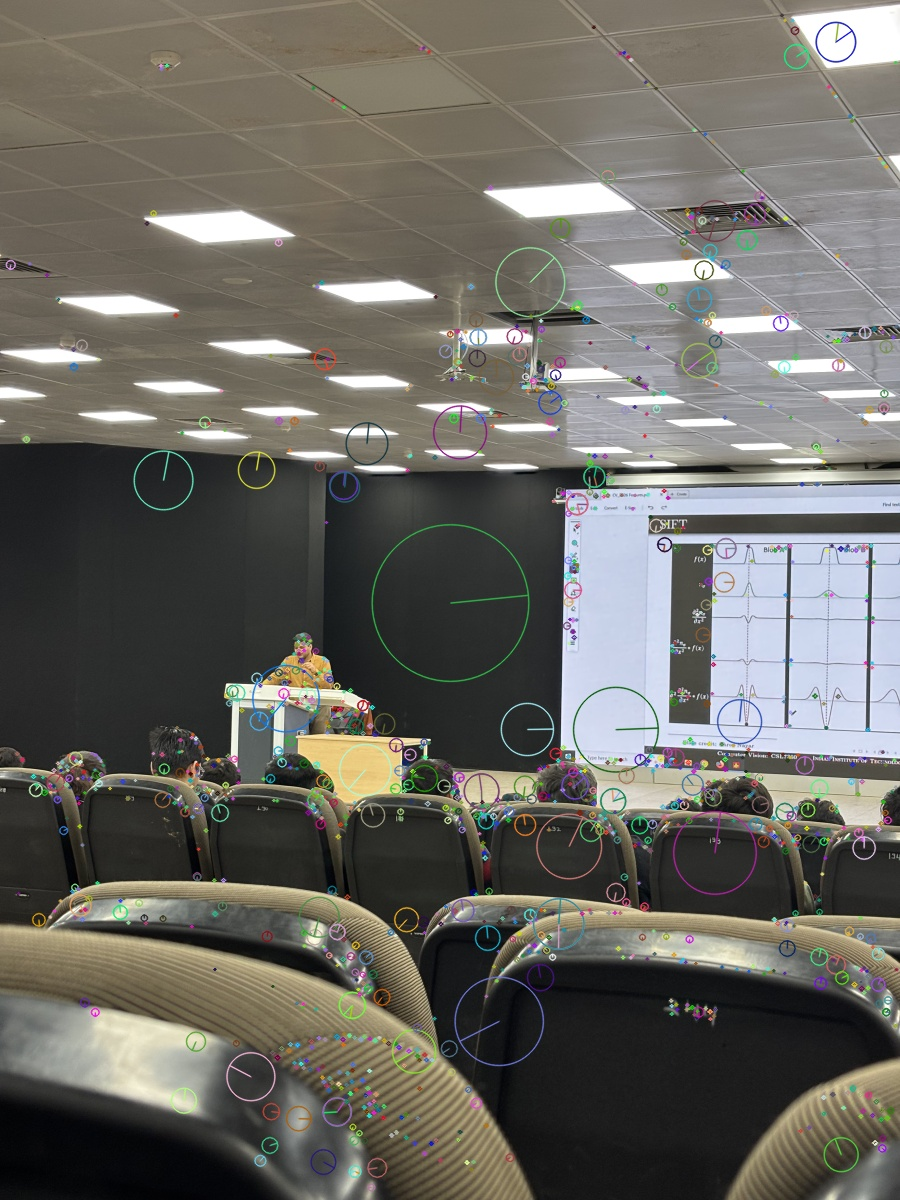
\includegraphics[width=0.48\linewidth]{keypoints_0.jpg}%
  }\hfill
  \subfloat[SIFT keypoints --- Centre image]{%
    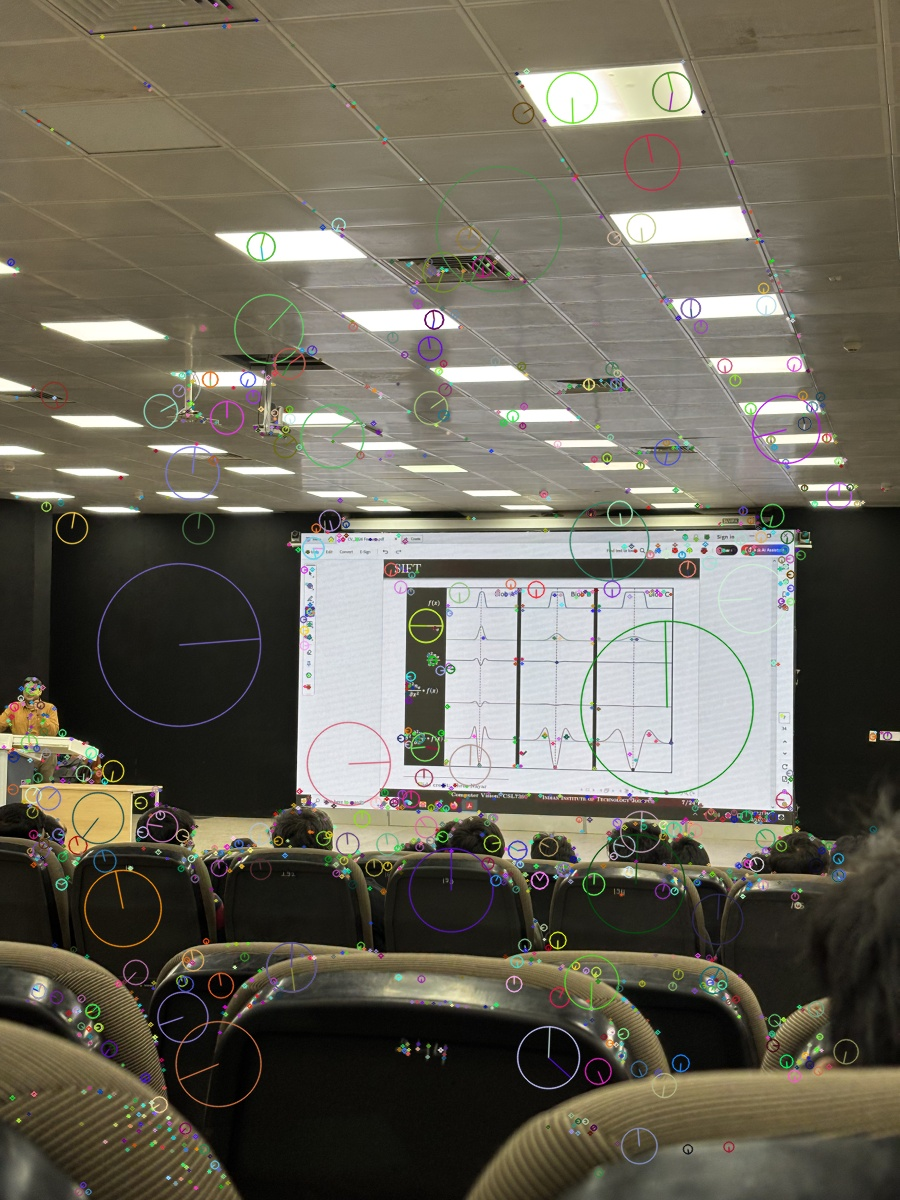
\includegraphics[width=0.48\linewidth]{keypoints_1.jpg}%
  }
  \caption{SIFT keypoint visualisation. Circle radii indicate scale; lines
           indicate dominant orientation.}
  \label{fig:keypoints}
\end{figure}

\begin{figure}[!t]
  \centering
  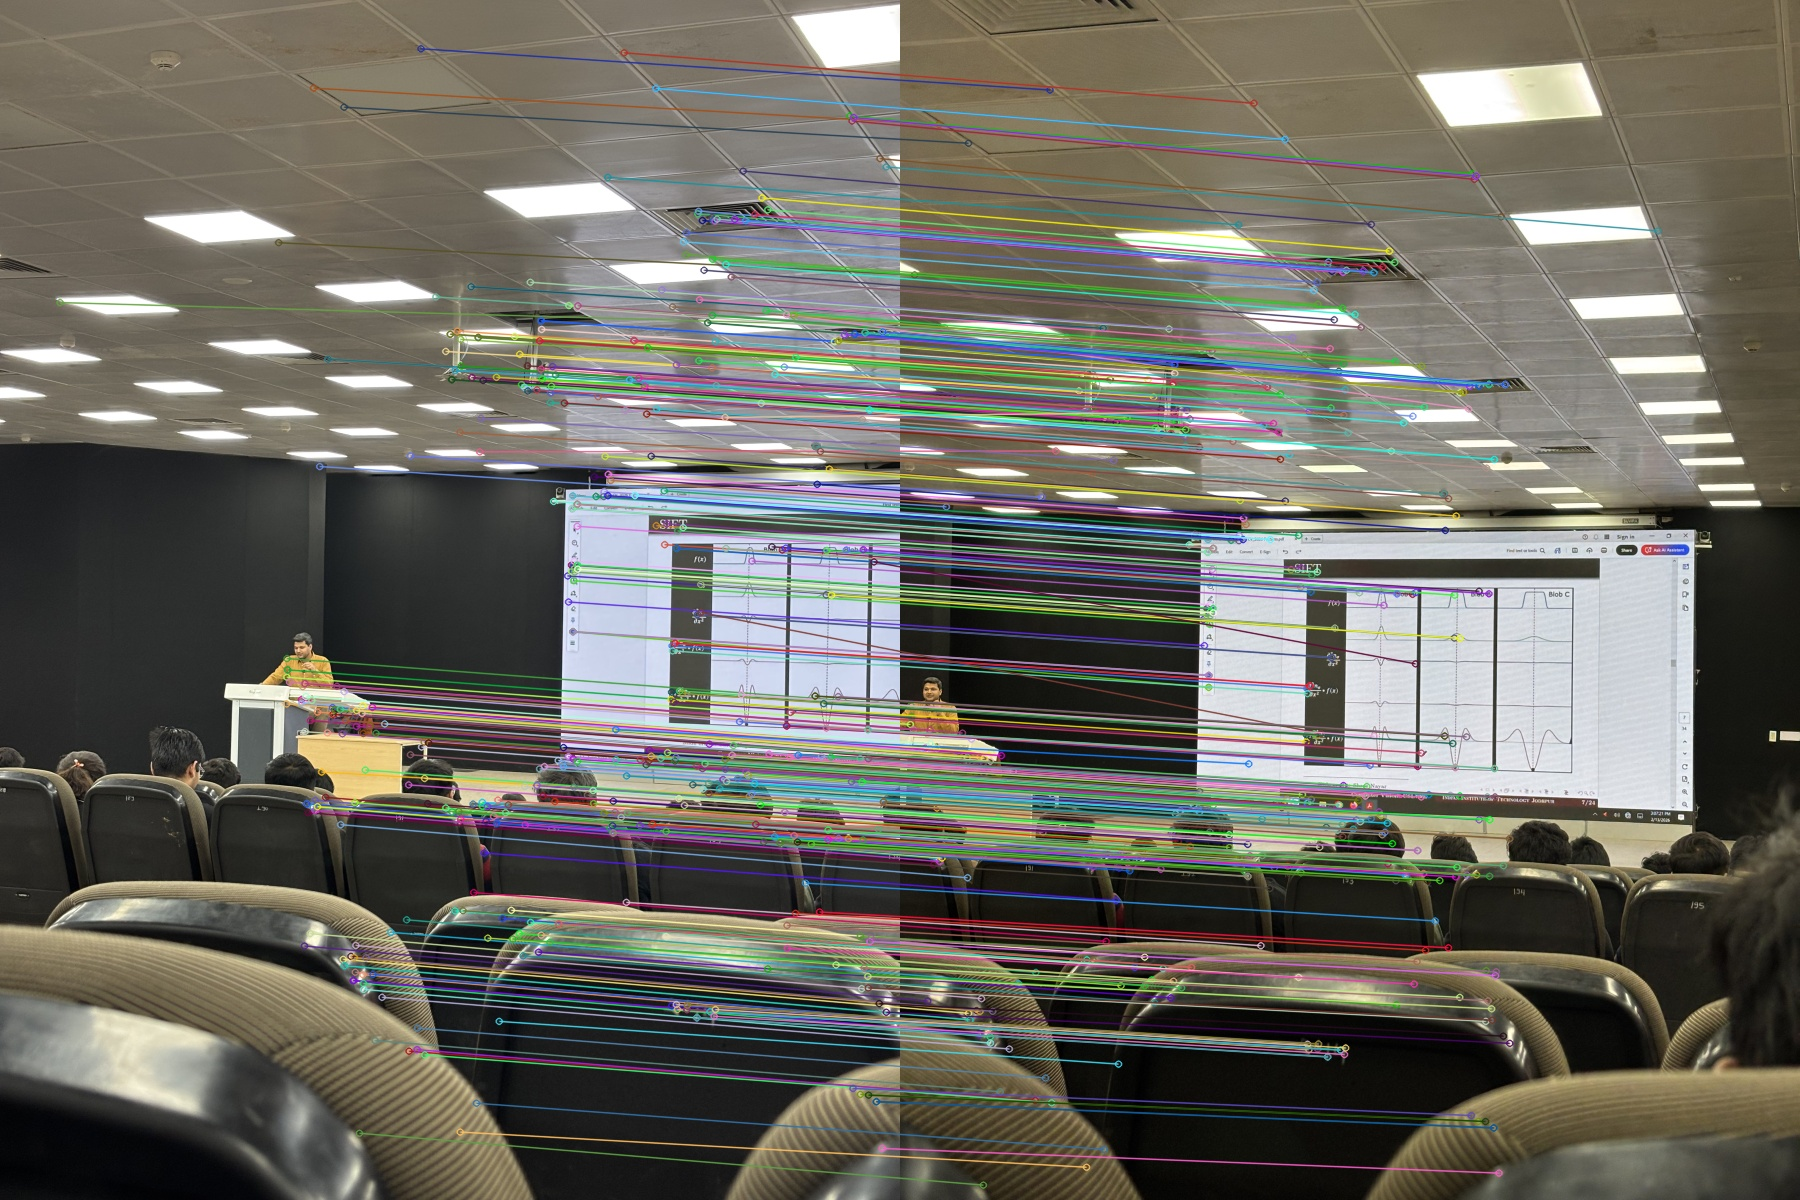
\includegraphics[width=0.95\linewidth]{matches_0-1.jpg}
  \caption{Feature matches between left and centre images after Lowe's ratio
           test (about 485 matches shown).}
  \label{fig:matches01}
\end{figure}

\begin{figure}[!t]
  \centering
  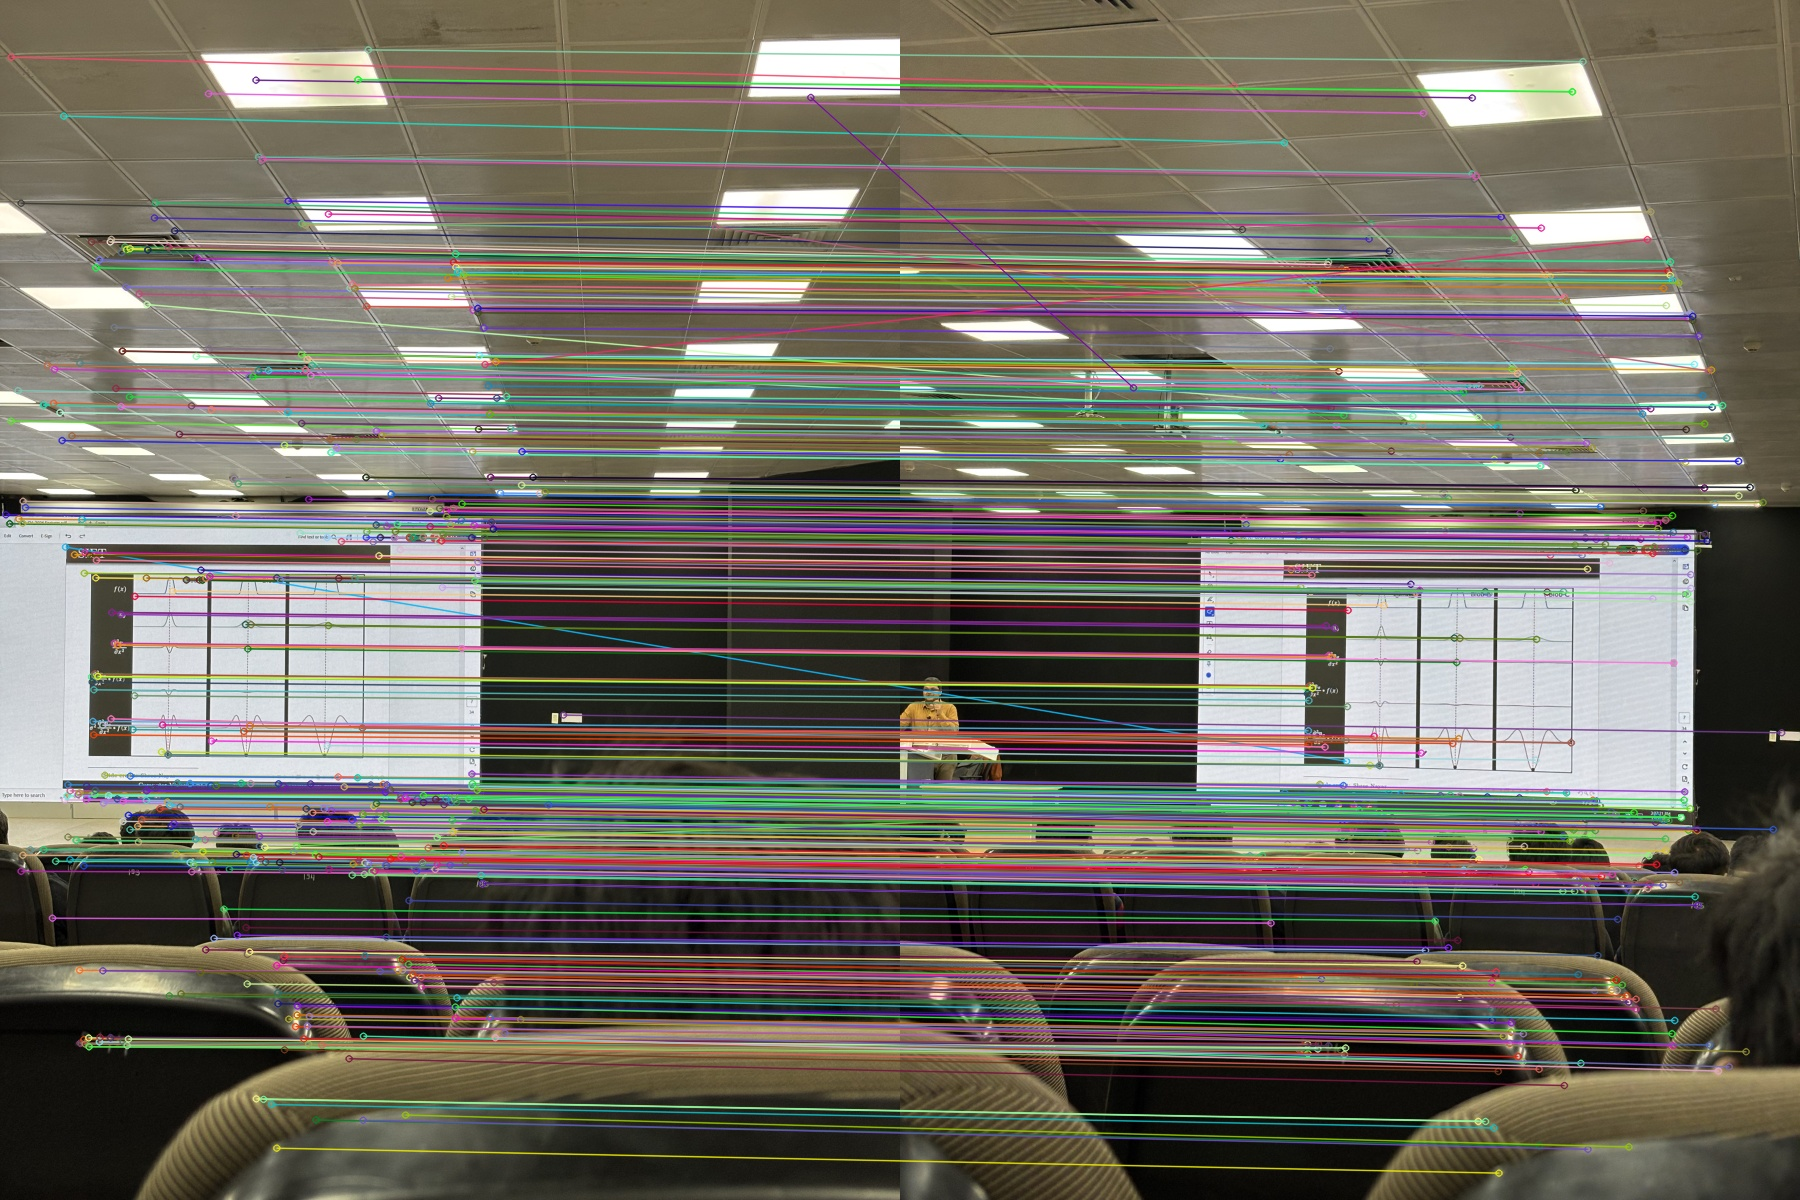
\includegraphics[width=0.95\linewidth]{matches_2-1.jpg}
  \caption{Feature matches between right and centre images (about 717 matches).}
  \label{fig:matches21}
\end{figure}

\subsection{Warping Results}

After homography estimation, each image is warped onto the common canvas
(Figure~\ref{fig:warped}). The centre image remains the reference frame, while
left and right images are perspectively transformed and then locally refined by
ECC to reduce residual overlap misalignment.

\begin{figure}[!t]
  \centering
  \subfloat[Warped left]{%
    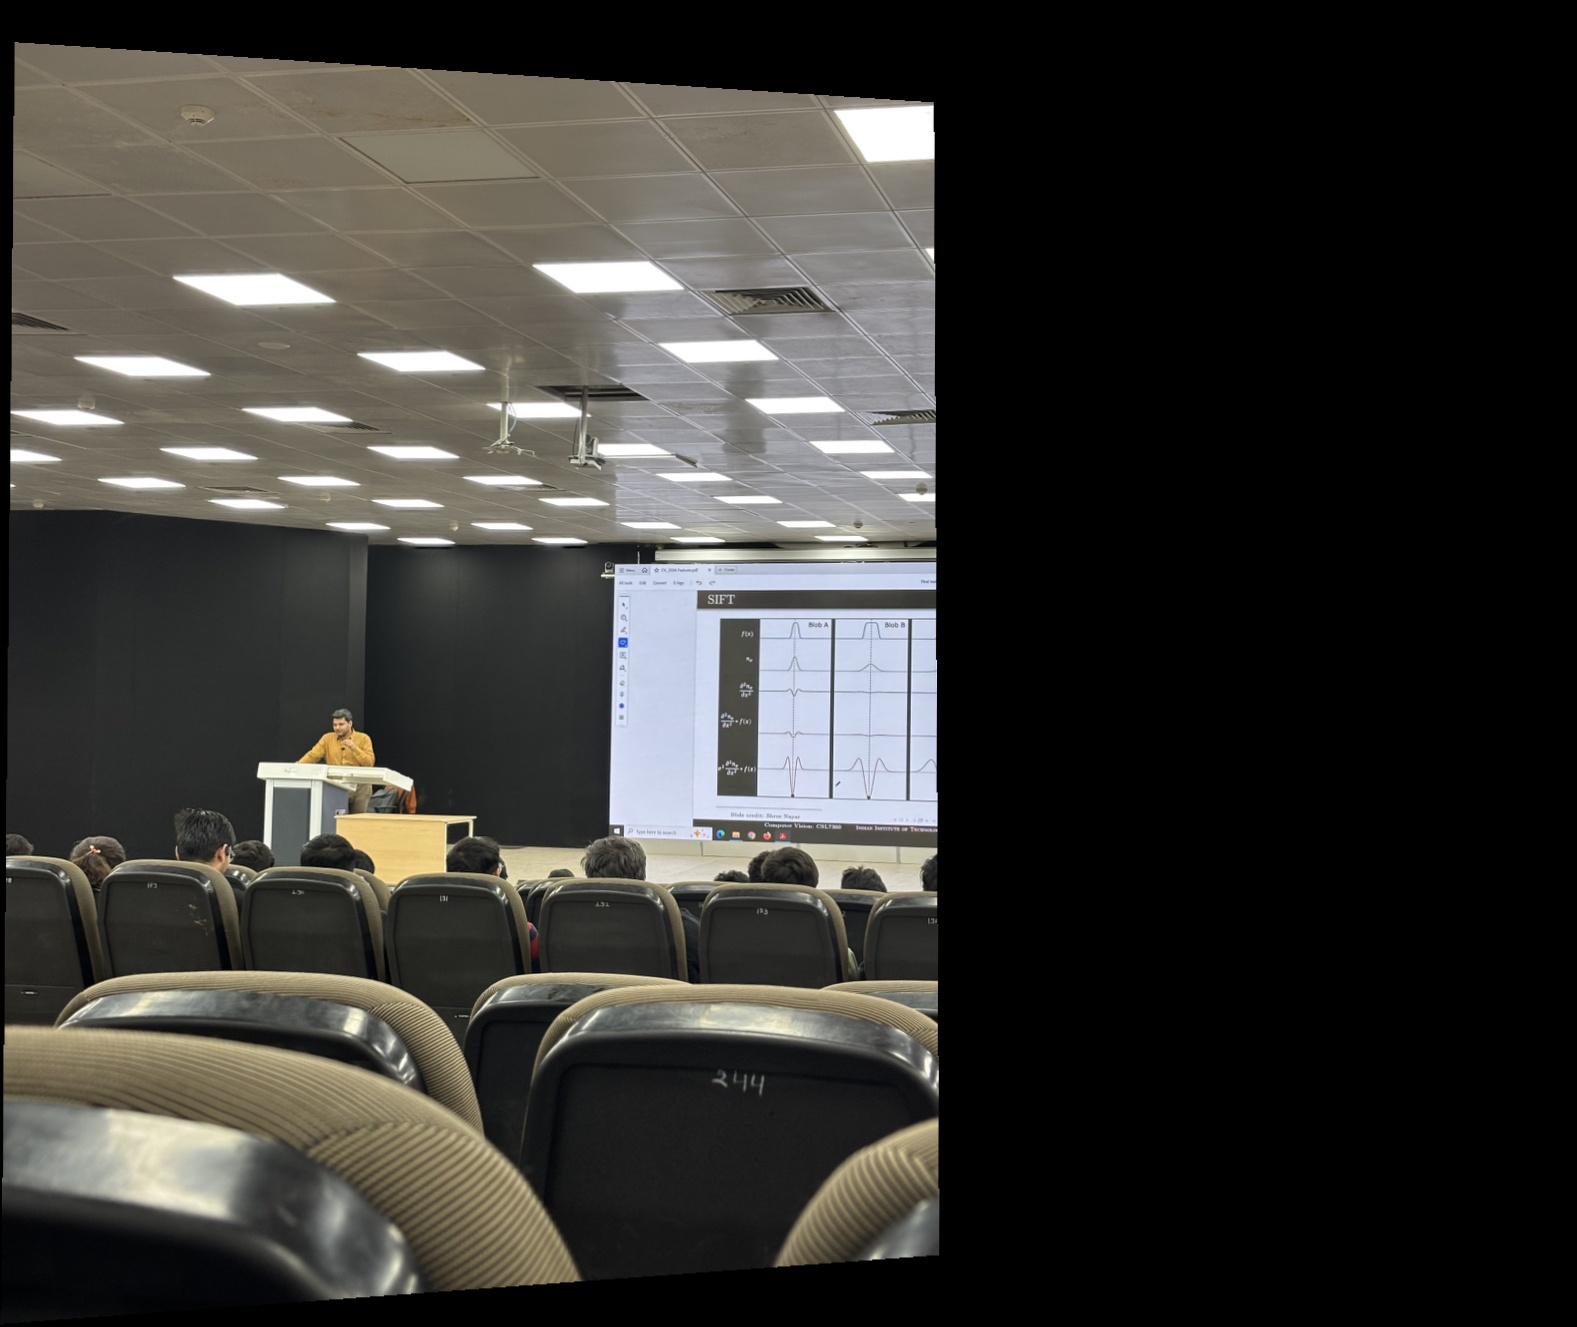
\includegraphics[width=0.32\linewidth]{warped_0.jpg}%
  }\hfill
  \subfloat[Warped centre]{%
    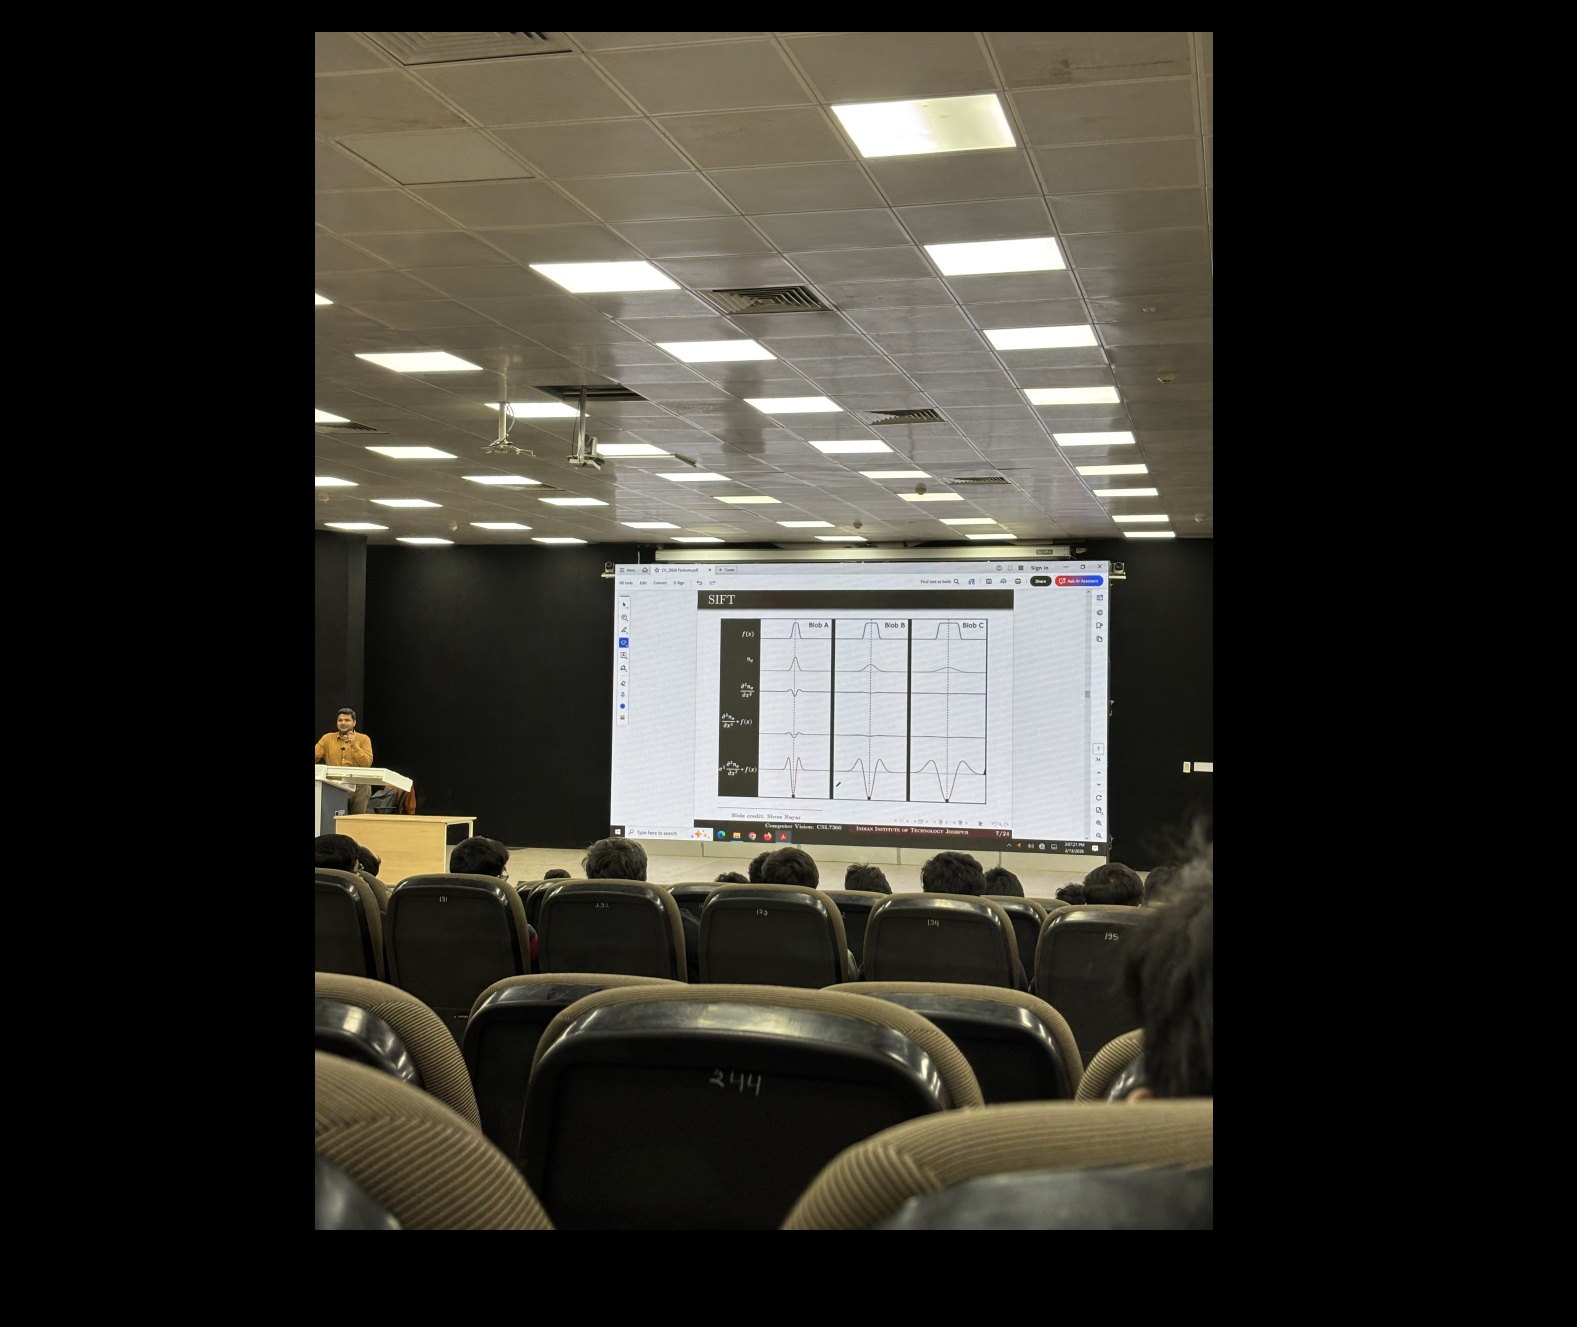
\includegraphics[width=0.32\linewidth]{warped_1.jpg}%
  }\hfill
  \subfloat[Warped right]{%
    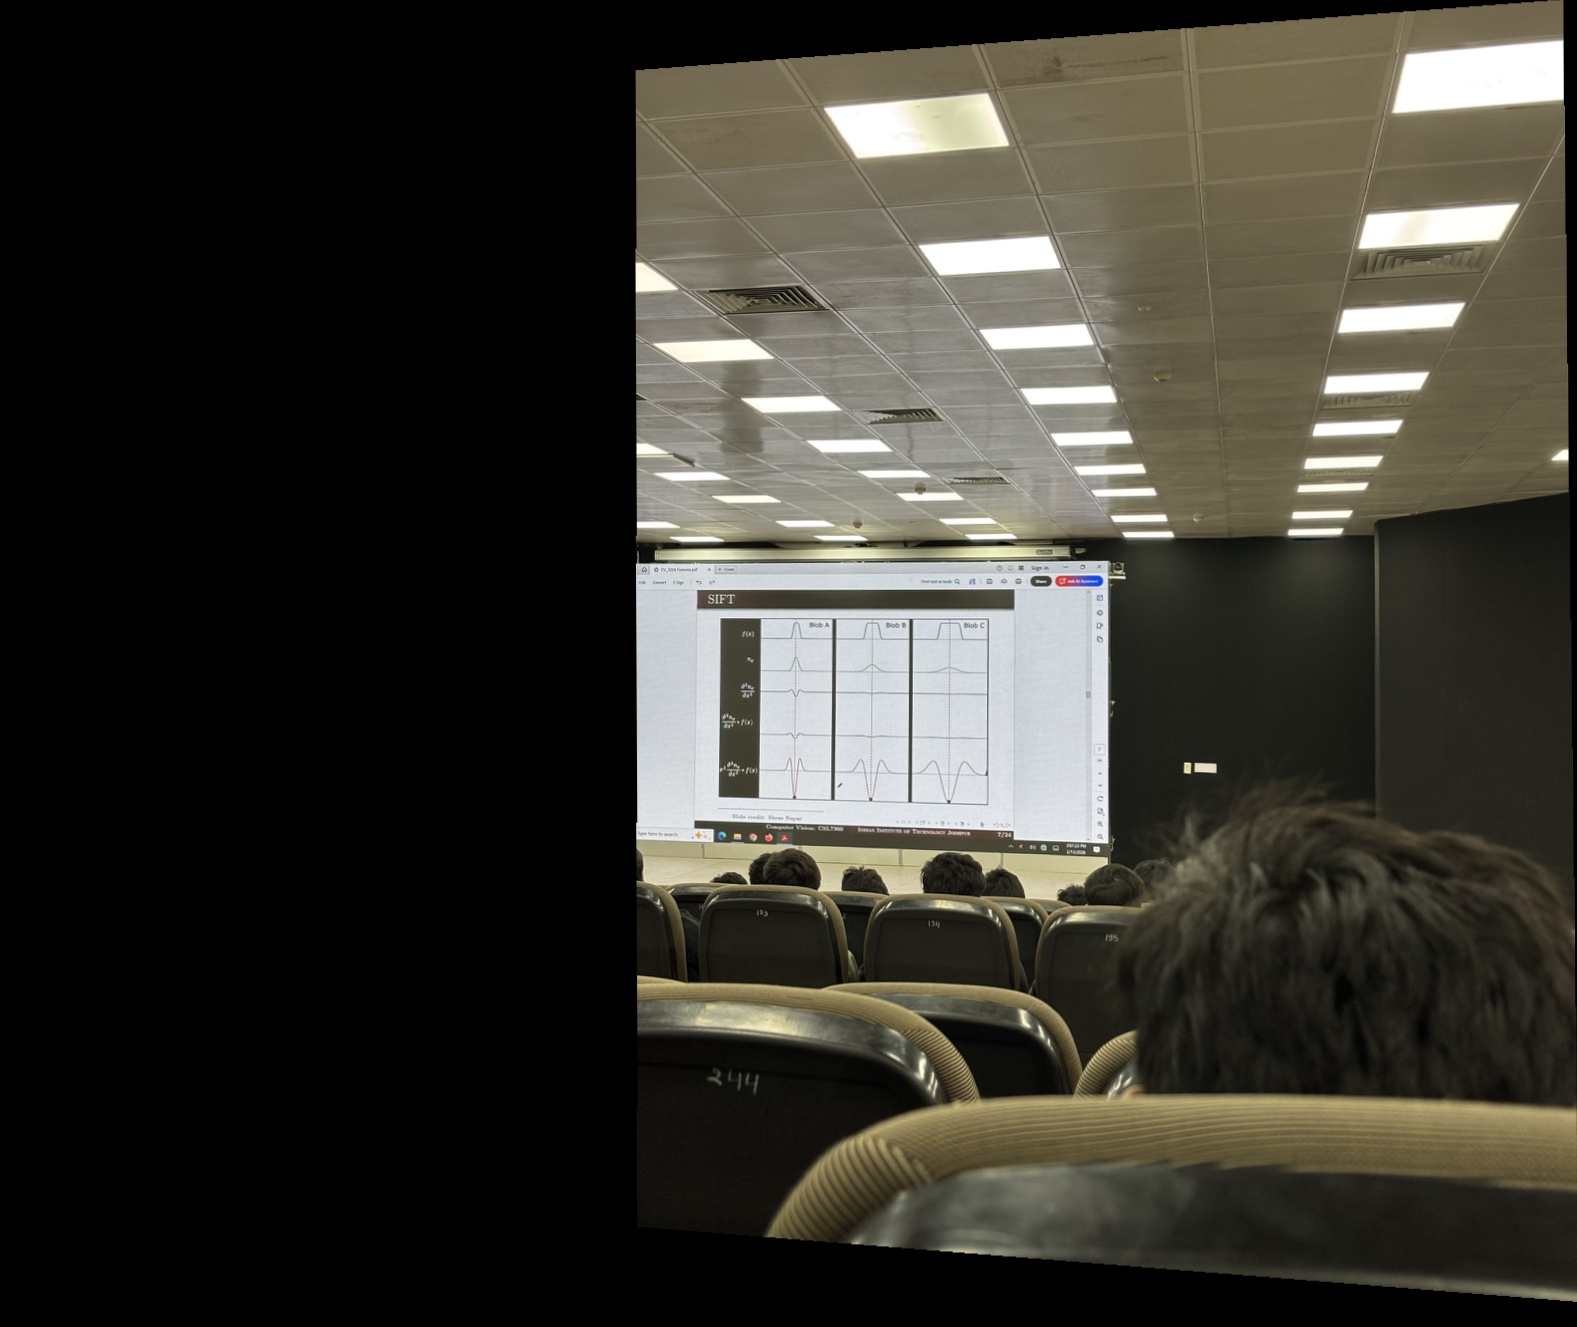
\includegraphics[width=0.32\linewidth]{warped_2.jpg}%
  }
  \caption{All three images warped onto the common canvas via their respective homographies.}
  \label{fig:warped}
\end{figure}

\subsection{Cylindrical Projection}

Figure~\ref{fig:cylindrical} shows the cylindrical projections of the input
images.  Note that unlike planar warping, the cylindrical projection
introduces barrel-like curvature but avoids the extreme stretching at the
edges that planar homographies cause.

\begin{figure}[!t]
  \centering
  \subfloat[Cylindrical left]{%
    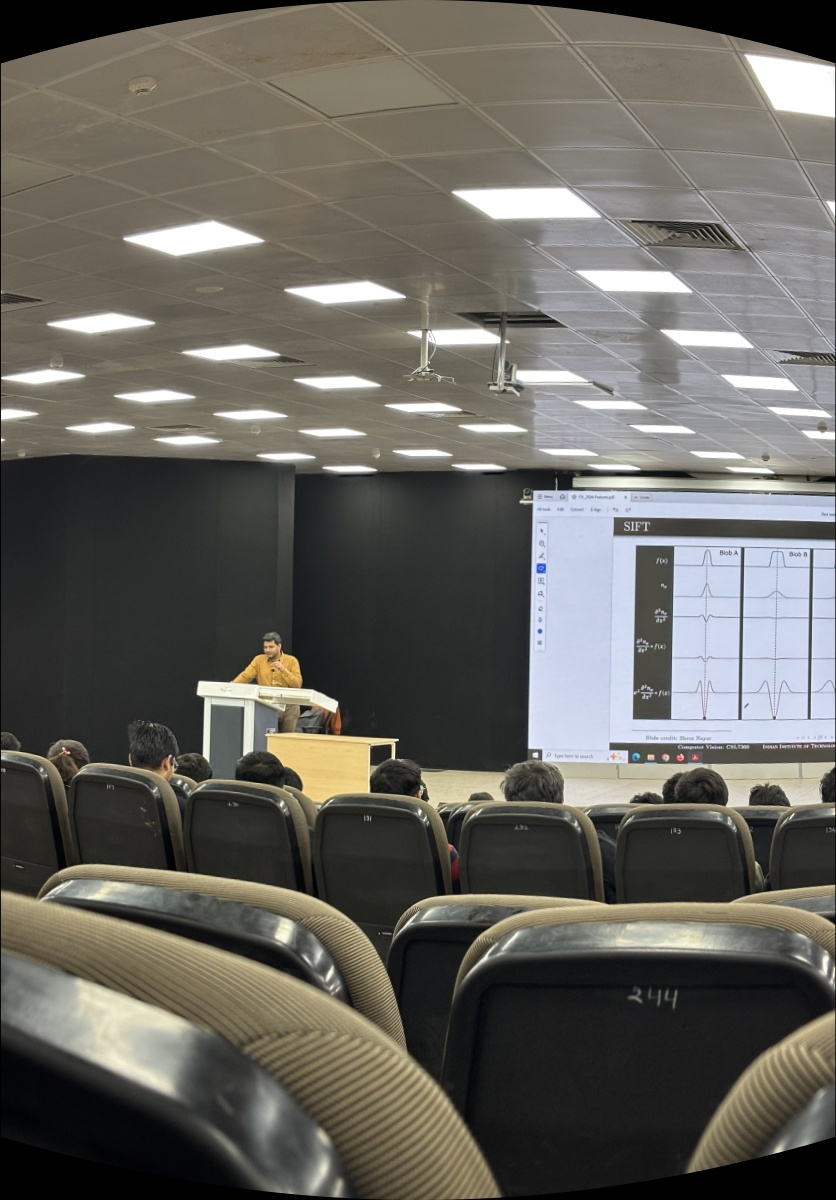
\includegraphics[width=0.32\linewidth]{cylindrical_0.jpg}%
  }\hfill
  \subfloat[Cylindrical centre]{%
    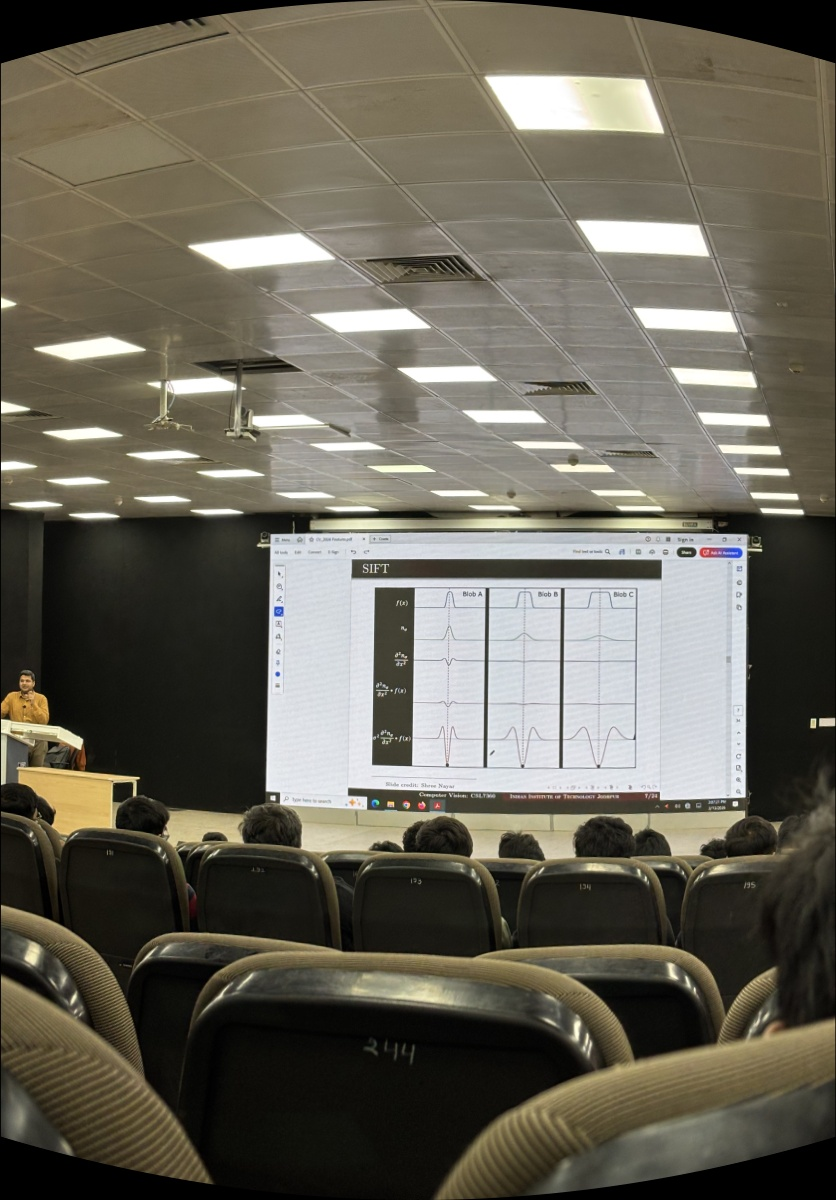
\includegraphics[width=0.32\linewidth]{cylindrical_1.jpg}%
  }\hfill
  \subfloat[Cylindrical right]{%
    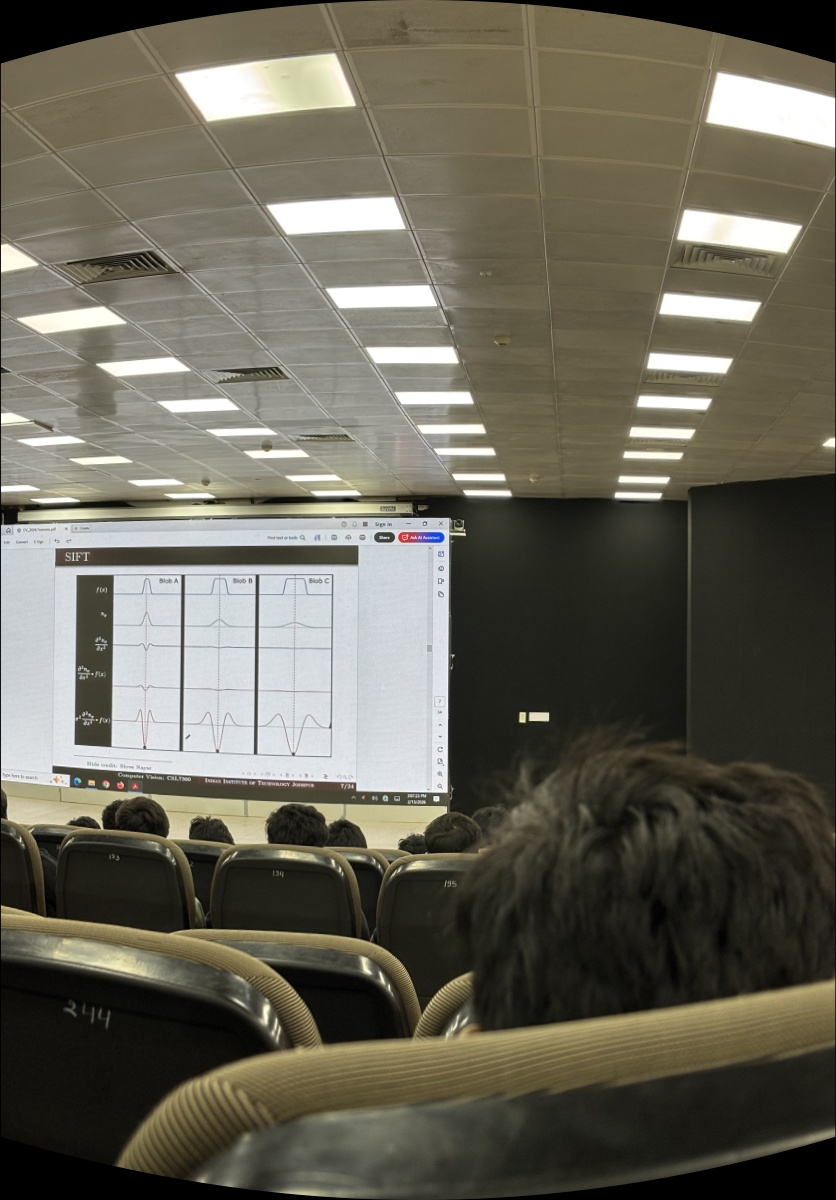
\includegraphics[width=0.32\linewidth]{cylindrical_2.jpg}%
  }
  \caption{Images projected onto a cylindrical surface ($f = w$ pixels).
           Vertical lines remain straight; horizontal curvature replaces
           the planar edge distortion.}
  \label{fig:cylindrical}
\end{figure}

\subsection{Blending Comparison}

Figure~\ref{fig:comparison} shows outputs after ECC refinement and adaptive
deghost blending. Compared with naive overwrite, both linear and multi-band
modes substantially reduce ghosting and seam visibility in the monitor/desk
overlap. Cylindrical projection still helps geometric distortion for wider
views, but in this close-range scene the planar path with deghosting gives the
best perceptual result.

\subsubsection{Quantitative Metrics}

Table~\ref{tab:blend-metrics} summarises quantitative metrics for three
blending strategies. Higher PSNR/SSIM indicates stronger fidelity in the
overlap region, while lower seam gradient and colour consistency indicate
smoother, more exposure-consistent transitions; edge variance serves as a
proxy for detail preservation.

\begin{table}[!t]
  \centering
  \footnotesize
  \setlength{\tabcolsep}{4pt} % reduce column spacing
  \renewcommand{\arraystretch}{1.05} % tighten row spacing
  \caption{Quantitative comparison on the challenging \texttt{iv2} set.}
  \label{tab:blend-metrics}
  \begin{tabular}{lccc}
    \toprule
    \textbf{Metric} & \textbf{Naive} & \textbf{Linear} & \textbf{Multi-Band} \\
    \midrule
    PSNR (dB)$\,\uparrow$ & 18.94 & 25.70 & 25.70 \\
    SSIM$\,\uparrow$ & 0.8281 & 0.9255 & 0.9255 \\
    Seam Grad.$\,\downarrow$ & 55.99 & 41.76 & 41.76 \\
    Edge Var.$\,\uparrow$ & 579.96 & 632.87 & 632.87 \\
    Colour Cons.$\,\downarrow$ & 36.64 & 57.44 & 57.44 \\
    Time (s) & 0.0970 & 0.1625 & 0.1570 \\
    \bottomrule
  \end{tabular}
\end{table}



On this parallax-heavy set, naive stitching performs worst by a wide margin.
The ECC + adaptive deghost pipeline raises PSNR from 18.94 to 25.70 and
reduces seam gradient from 55.99 to 41.76. In this run, both linear and
multi-band branches selected the same strong deghost path, yielding nearly
identical outputs and metrics.

\begin{figure}[!t]
  \centering
  \subfloat[Naive stitch --- visible seams]{%
    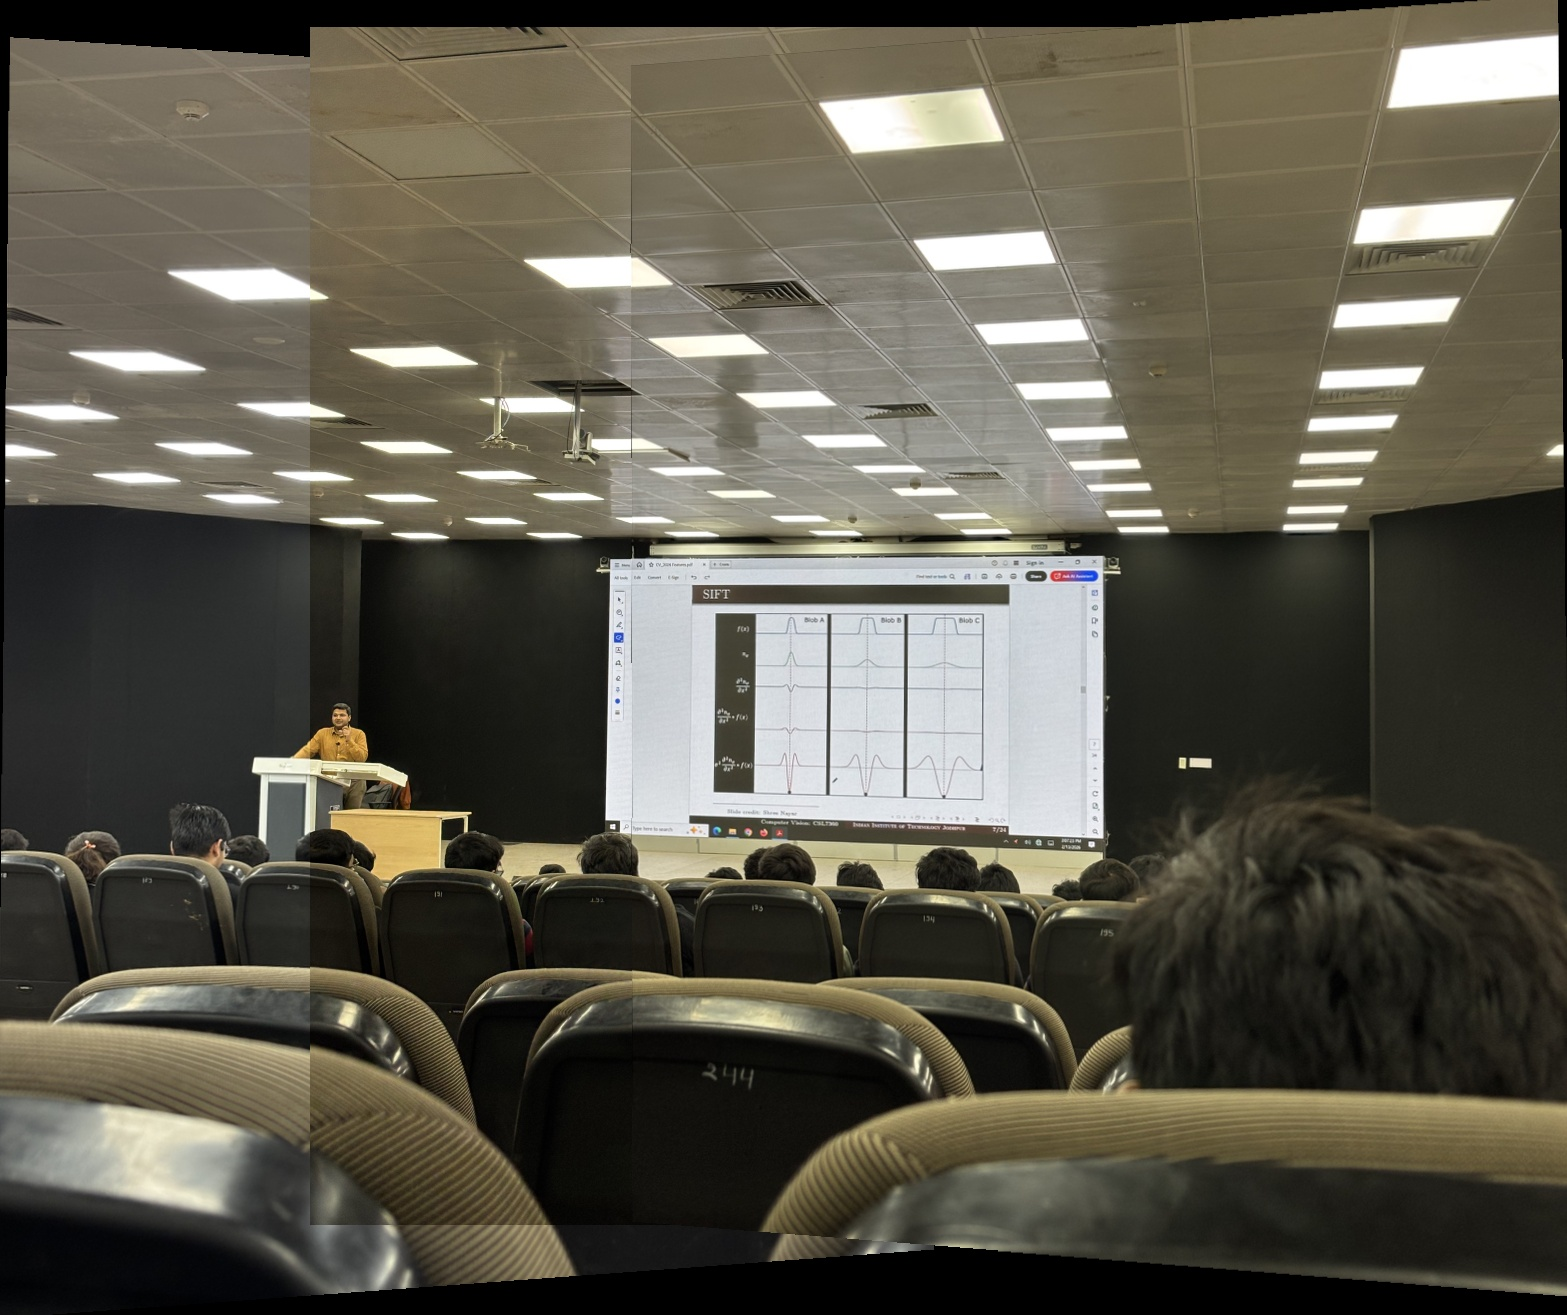
\includegraphics[width=0.24\linewidth]{naive_stitch.jpg}%
  }\hfill
  \subfloat[Linear feathering blend]{%
    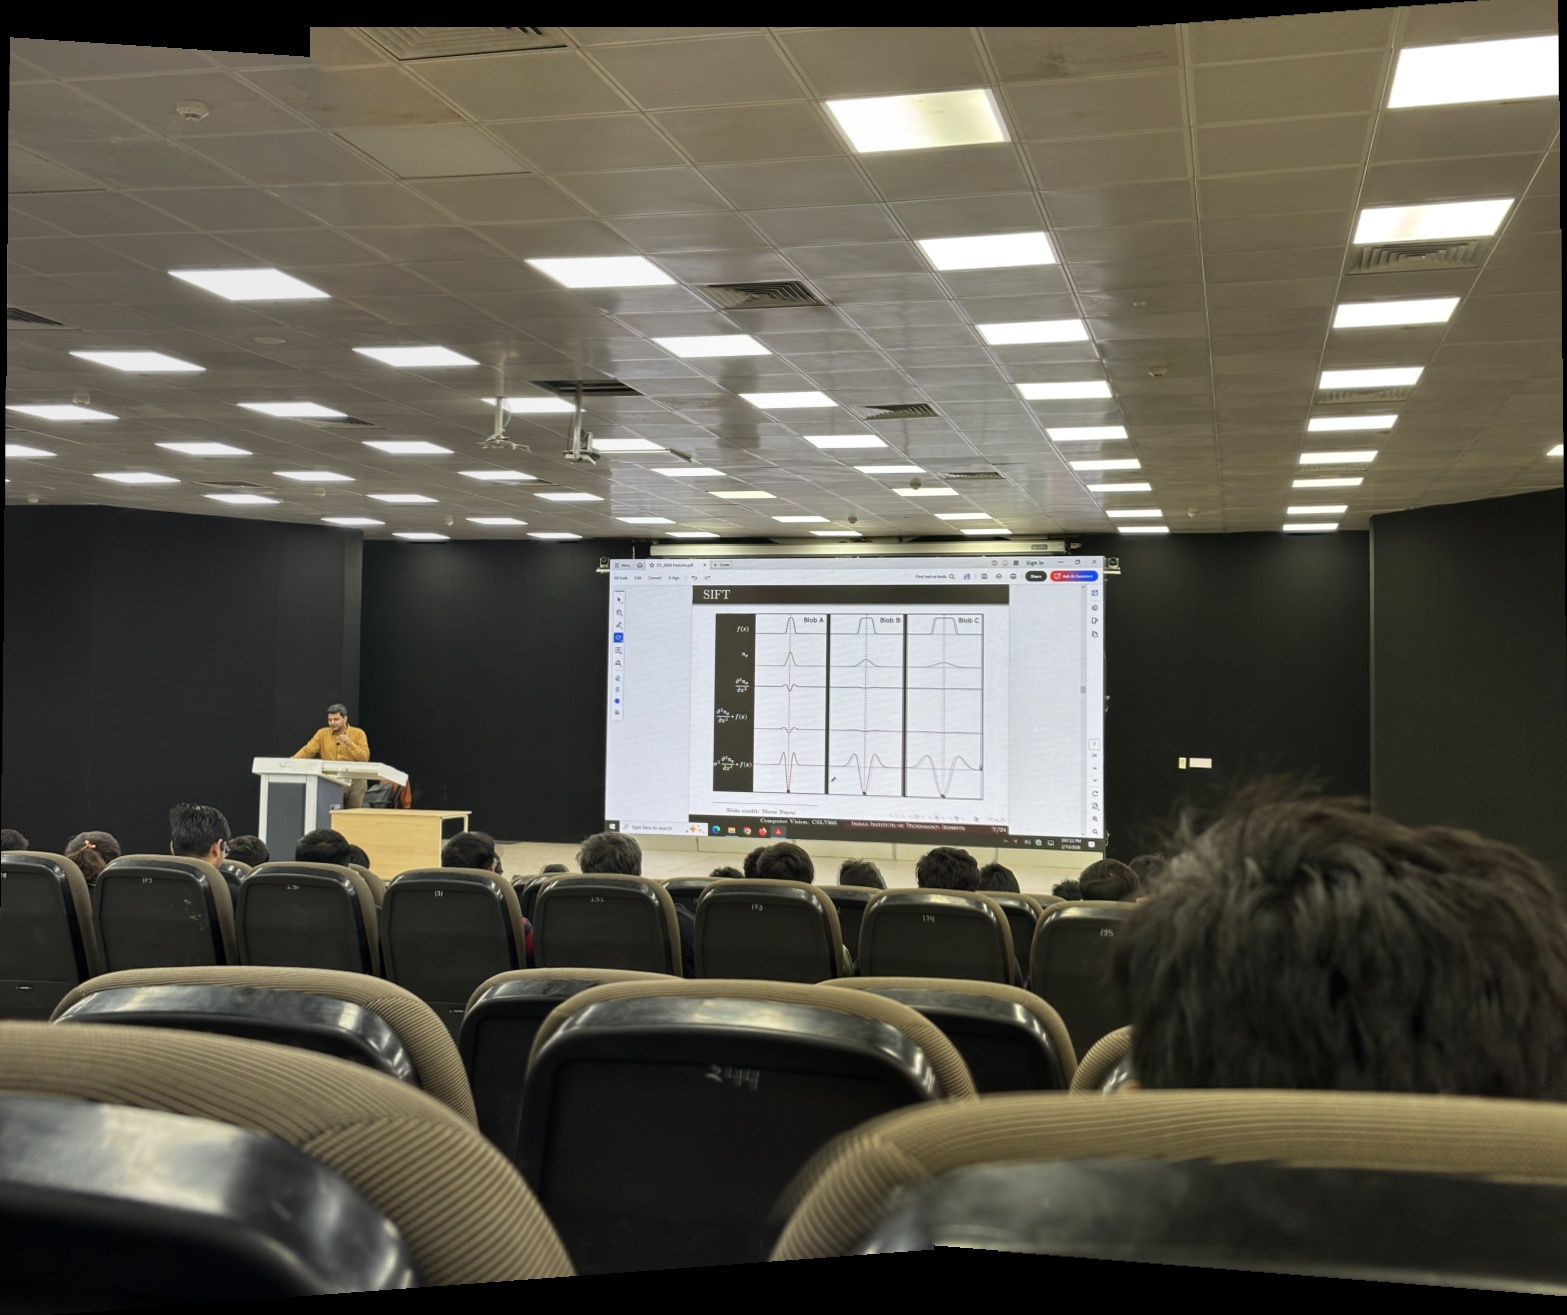
\includegraphics[width=0.24\linewidth]{panorama_linear.jpg}%
  }\hfill
  \subfloat[Multi-band blending (Laplacian pyramid)]{%
    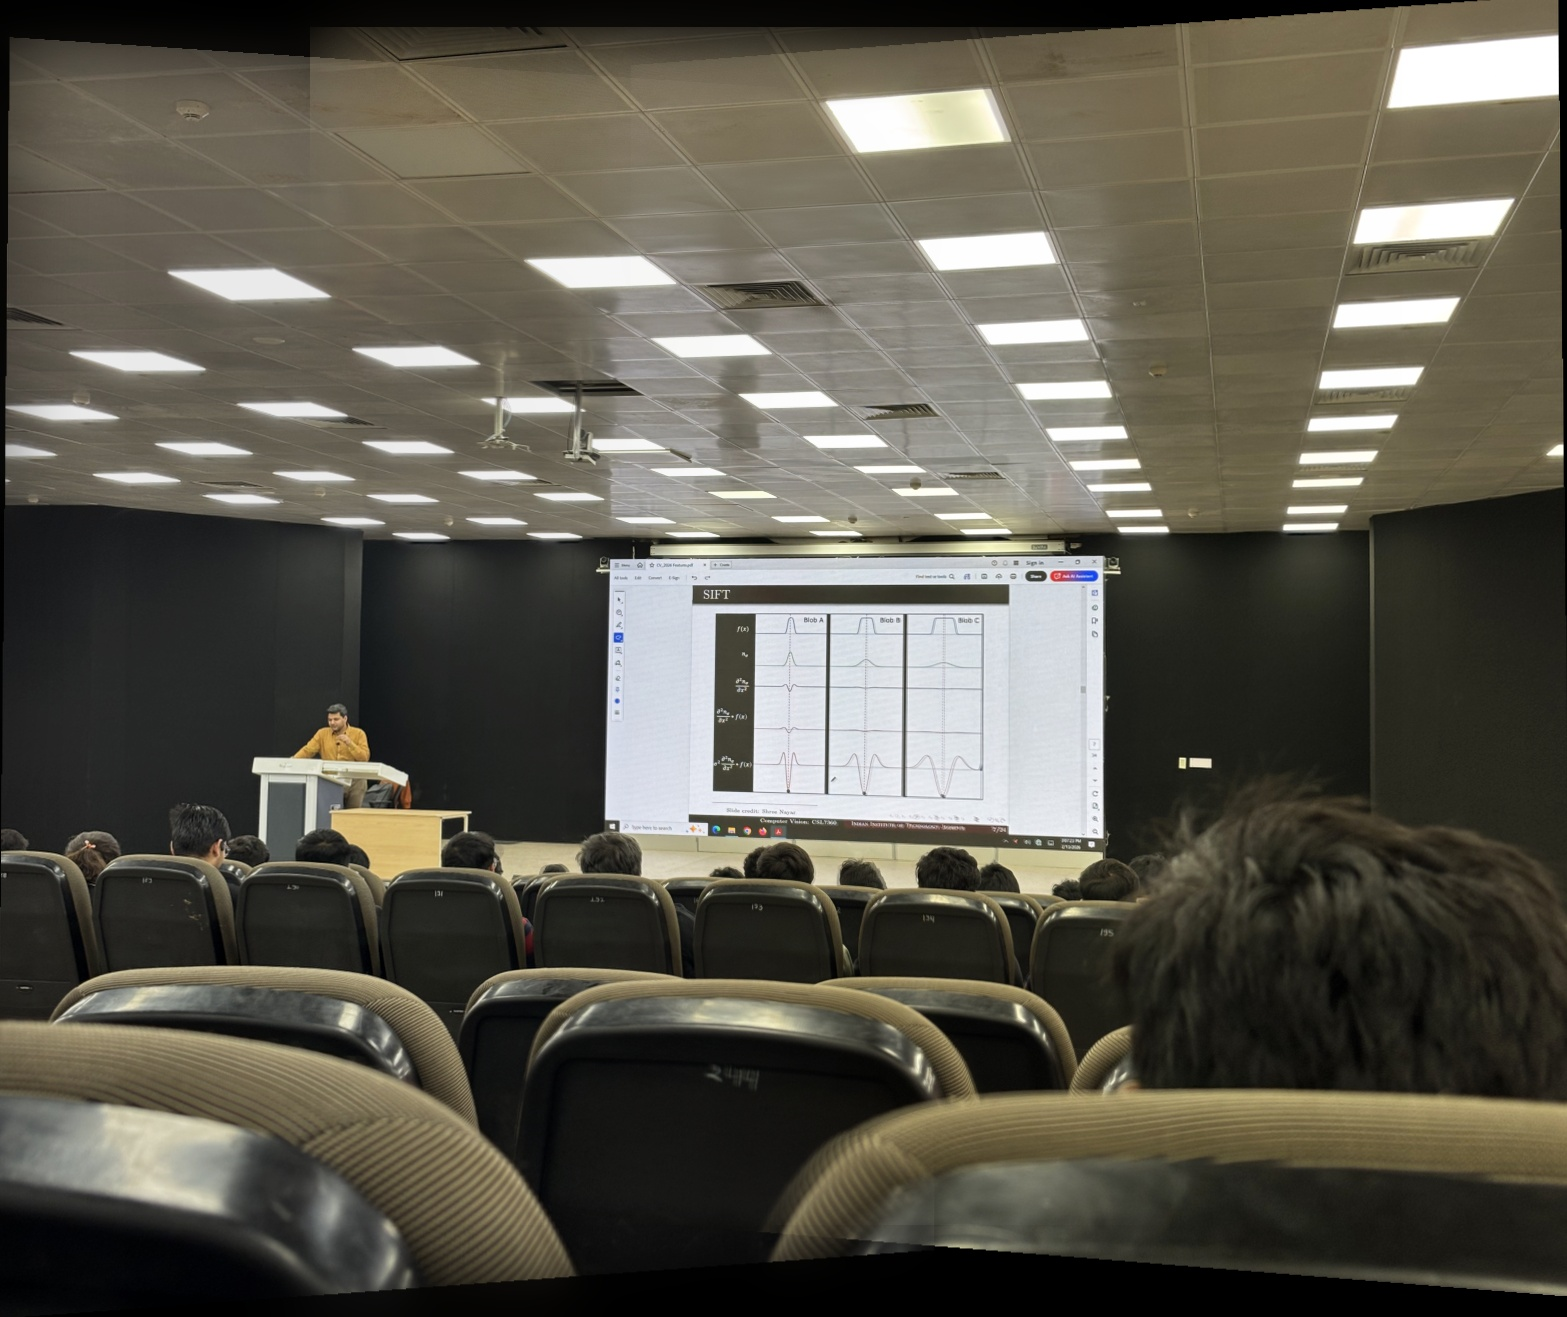
\includegraphics[width=0.24\linewidth]{panorama_multiband.jpg}%
  }\hfill
  \subfloat[Cylindrical warp + multi-band blending]{%
    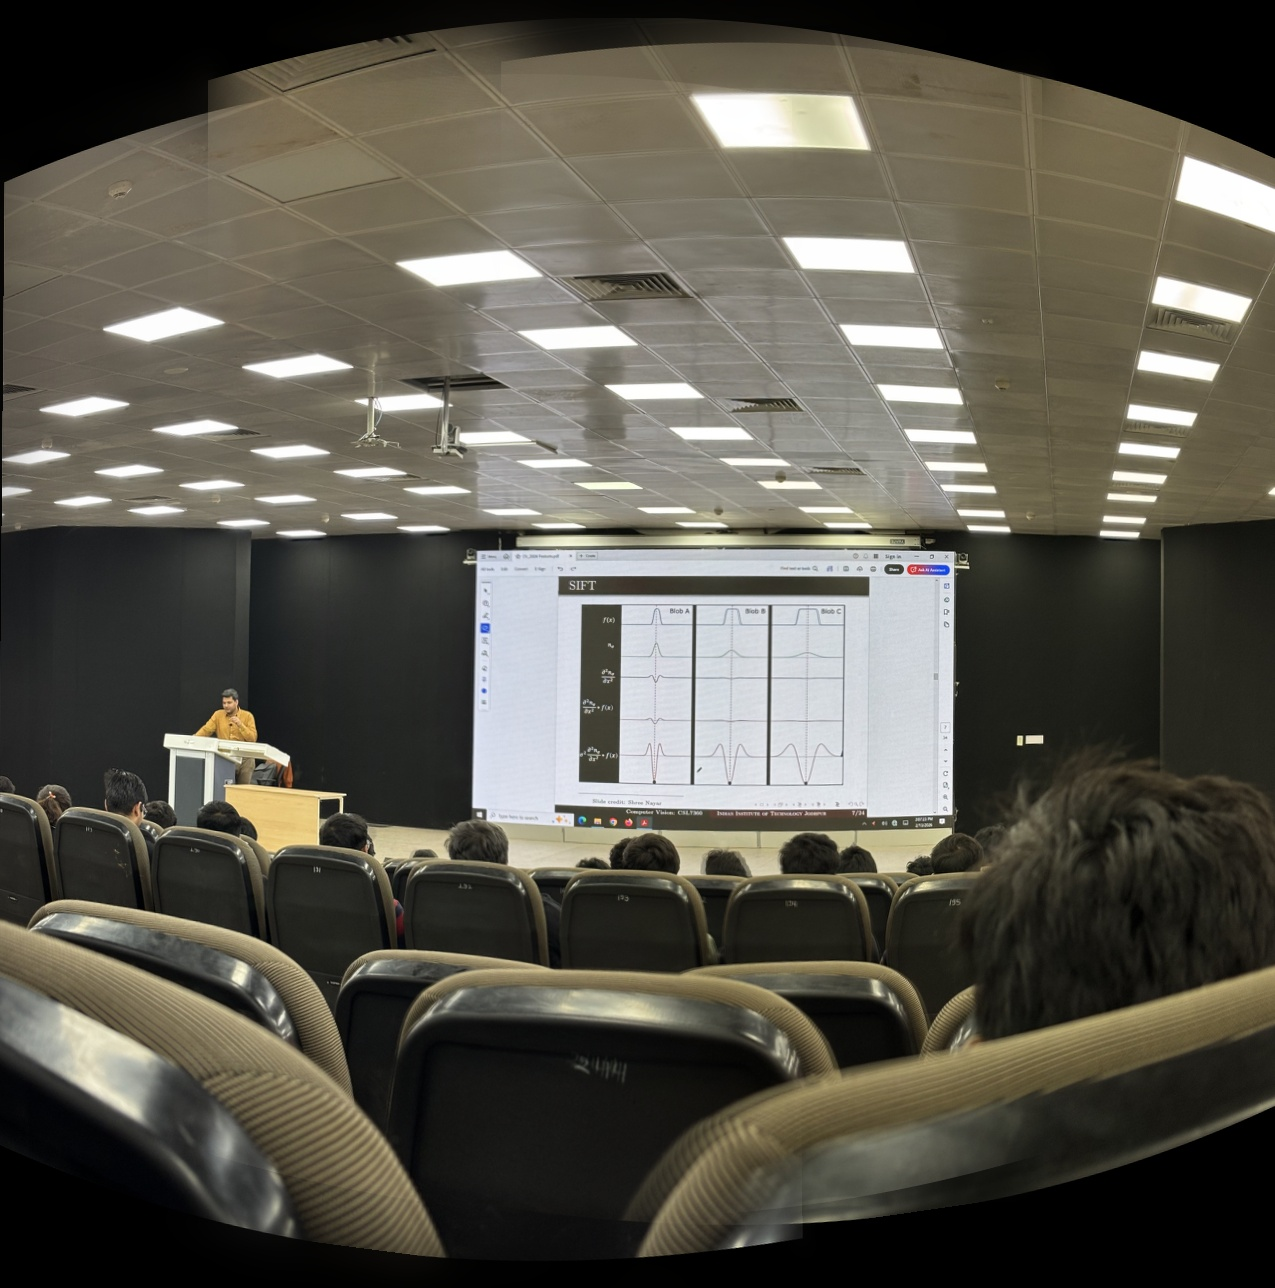
\includegraphics[width=0.24\linewidth]{panorama_cylindrical.jpg}%
  }
  \caption{Comparison of all stitching and blending methods after the pipeline
           updates. Ghosting is substantially reduced in (b) and (c).}
  \label{fig:comparison}
\end{figure}

\subsection{Timing}

For the resized 900$\times$1200 input images, the complete run (\texttt{--method all})
takes about \textbf{5.8 s} on the current machine, including keypoint
extraction, matching, homography estimation, ECC refinement, and all output
renders.

\begin{table}[!t]
  \centering
  \caption{Pipeline Execution Summary}
  \label{tab:timing}
  \begin{tabular}{lcc}
    \toprule
    \textbf{Method} & \textbf{Output Size} & \textbf{Quality} \\
    \midrule
    Naive Stitch           & 1644$\times$1413 & Strong ghosting/seams  \\
    Linear Feathering      & 1644$\times$1413 & Deghosted (adaptive)   \\
    Multi-Band Blend       & 1644$\times$1413 & Deghosted (adaptive)   \\
    Cylindrical + MB       & 1335$\times$1218 & Lower edge distortion  \\
    \bottomrule
  \end{tabular}
\end{table}


% ═══════════════════════════════════════════════════════════════════════════
%   5. SOFTWARE ARCHITECTURE
% ═══════════════════════════════════════════════════════════════════════════
\FloatBarrier
\section{Software Architecture}
\label{sec:code}

The codebase is organised as a modular Python package for maintainability
and reuse:

\begin{table}[!t]
  \centering
  \caption{Codebase modules and responsibilities.}
  \label{tab:modules}
  \begin{tabular}{p{0.46\columnwidth}p{0.46\columnwidth}}
    \toprule
    \textbf{Module} & \textbf{Responsibility} \\
    \midrule
    \texttt{src/config.py}     & Tuneable constants \\
    \texttt{src/features.py}   & SIFT detection and FLANN matching \\
    \texttt{src/homography.py} & Homography estimation (RANSAC) \\
    \texttt{src/warping.py}    & Perspective and cylindrical warping \\
    \texttt{src/blending.py}   & Naive, linear, multi-band blending \\
    \texttt{src/utils.py}      & I/O, gain compensation, cropping \\
    \texttt{panorama\_stitcher.py}  & CLI entry point and pipelines \\
    \bottomrule
  \end{tabular}
\end{table}

The entry point supports multiple methods via CLI flags:
\begin{lstlisting}
python panorama_stitcher.py --images_dir images/ \
                            --method all
\end{lstlisting}


% ═══════════════════════════════════════════════════════════════════════════
%   6. CONCLUSION
% ═══════════════════════════════════════════════════════════════════════════
\section{Conclusion}
\label{sec:conclusion}

We presented a complete and modular panorama stitching pipeline that covers
the classical approach (SIFT + RANSAC homography + blending) and three
advanced techniques. Key findings:

\begin{itemize}
  \item \textbf{ECC local refinement} is crucial when one image pair has weaker
        geometric consensus; it significantly reduces residual misalignment
        before blending.
  \item \textbf{Adaptive deghost seam blending} is more reliable than pure
        averaging for near-field parallax scenes, reducing double edges around
        objects like cables and monitor boundaries.
  \item \textbf{Cylindrical warping} is essential for wide-angle stitching,
        removing the severe edge distortion caused by planar homographies.
  \item \textbf{Centre-referenced alignment} (choosing the middle image as
        the reference) distributes alignment error symmetrically, avoiding
        the drift that accumulates when chaining homographies sequentially
        from one end.
\end{itemize}

Future work could explore \textbf{bundle adjustment} for global optimisation
of all camera parameters, \textbf{exposure fusion} for HDR panoramas, and
\textbf{content-aware seam selection} via graph cuts~\cite{kwatra2003}.

% ═══════════════════════════════════════════════════════════════════════════
%   REFERENCES
% ═══════════════════════════════════════════════════════════════════════════
\begin{thebibliography}{10}

\bibitem{lowe2004}
D.~G. Lowe, ``Distinctive image features from scale-invariant keypoints,''
\emph{International Journal of Computer Vision}, vol.~60, no.~2,
pp.~91--110, 2004.

\bibitem{muja2009}
M.~Muja and D.~G. Lowe, ``Fast approximate nearest neighbors with automatic
algorithm configuration,'' in \emph{Proc. International Conference on
Computer Vision Theory and Applications (VISAPP)}, 2009, pp.~331--340.

\bibitem{fischler1981}
M.~A. Fischler and R.~C. Bolles, ``Random sample consensus: A paradigm for
model fitting with applications to image analysis and automated cartography,''
\emph{Communications of the ACM}, vol.~24, no.~6, pp.~381--395, 1981.

\bibitem{burt1983}
P.~J. Burt and E.~H. Adelson, ``A multiresolution spline with application to
image mosaics,'' \emph{ACM Transactions on Graphics}, vol.~2, no.~4,
pp.~217--236, 1983.

\bibitem{szeliski2006}
R.~Szeliski, ``Image alignment and stitching: A tutorial,'' \emph{Foundations
and Trends in Computer Graphics and Vision}, vol.~2, no.~1, pp.~1--104, 2006.

\bibitem{detone2018}
D.~DeTone, T.~Malisiewicz, and A.~Rabinovich, ``SuperPoint: Self-supervised
interest point detection and description,'' in \emph{Proc. CVPR Workshops},
2018.

\bibitem{sarlin2020}
P.-E. Sarlin, D.~DeTone, T.~Malisiewicz, and A.~Rabinovich, ``SuperGlue:
Learning feature matching with graph neural networks,'' in \emph{Proc. CVPR},
2020, pp.~4938--4947.

\bibitem{kwatra2003}
V.~Kwatra, A.~Sch{\"o}dl, I.~Essa, G.~Turk, and A.~Bobick, ``Graphcut
textures: Image and video synthesis using graph cuts,'' \emph{ACM Transactions
on Graphics}, vol.~22, no.~3, pp.~277--286, 2003.

\bibitem{brown2007}
M.~Brown and D.~G. Lowe, ``Automatic panoramic image stitching using
invariant features,'' \emph{International Journal of Computer Vision},
vol.~74, no.~1, pp.~59--73, 2007.

\bibitem{hartley2003}
R.~Hartley and A.~Zisserman, \emph{Multiple View Geometry in Computer Vision},
2nd~ed.\hskip 1em plus 0.5em minus 0.4em Cambridge University Press, 2003.

\end{thebibliography}

\end{document}
